\documentclass[11pt,a4paper,oneside]{report}

% ---------------------------------------------------------------------------
% Fill in before submission
\newcommand{\ReportAuthors}{Author Name (Roll No.)\\Author Name (Roll No.)}
\newcommand{\ReportCourse}{Optimization Methods for Machine Learning}
\newcommand{\ReportGuide}{Course Instructor}
\newcommand{\ReportDept}{Department Name}
\newcommand{\ReportInstitute}{Institute Name}
\newcommand{\ReportDate}{October 2026}
% ---------------------------------------------------------------------------

\usepackage{iftex}
\ifXeTeX
  \usepackage{fontspec}   % Latin Modern (OpenType) under XeLaTeX / Tectonic
\else
  \usepackage[T1]{fontenc}
  \usepackage[utf8]{inputenc}
  \usepackage{lmodern}
\fi
\usepackage[margin=1in]{geometry}
\usepackage{microtype}
\usepackage{amsmath,amssymb,amsthm,bm}
\usepackage{booktabs,tabularx,multirow,array}
\usepackage{graphicx}
\usepackage{caption,subcaption}
\usepackage{xcolor}
\usepackage{enumitem}
\usepackage{algorithm}
\usepackage{algpseudocode}
\usepackage{tikz}
\usetikzlibrary{arrows.meta,positioning,fit,calc,shapes.geometric}
\usepackage[numbers,sort&compress]{natbib}
\usepackage[hidelinks]{hyperref}
\usepackage{setspace}
\usepackage{fancyhdr}

\setstretch{1.15}
\setlist{itemsep=2pt,topsep=4pt}
\captionsetup{font=small,labelfont=bf}
\setlength{\parskip}{3pt}

\pagestyle{fancy}
\fancyhf{}
\fancyhead[L]{\small\nouppercase{\leftmark}}
\fancyfoot[C]{\thepage}
\renewcommand{\headrulewidth}{0.4pt}
\fancypagestyle{plain}{\fancyhf{}\fancyfoot[C]{\thepage}\renewcommand{\headrulewidth}{0pt}}

\theoremstyle{plain}
\newtheorem{proposition}{Proposition}[chapter]
\theoremstyle{definition}
\newtheorem{definition}{Definition}[chapter]
\theoremstyle{remark}
\newtheorem{remark}{Remark}[chapter]

\newcommand{\E}{\mathbb{E}}
\newcommand{\STOP}{\textsc{stop}}
\newcommand{\cand}{\mathcal{C}}
\newcommand{\gold}{\mathcal{G}}
\newcommand{\evid}{E}
\newcommand{\nTrain}{5,000}
\newcommand{\nVal}{1,000}
\newcommand{\nTest}{3,466}
\newcommand{\nTrainTables}{1,000}
\newcommand{\nValTables}{201}
\newcommand{\nTestTables}{3,053}
\newcommand{\testTablesInTrain}{262}
\newcommand{\testQuestionsWithTrainTable}{303}
\newcommand{\nTestTypeTable}{1,349}
\newcommand{\nTestTypePassage}{2,025}
\newcommand{\testReachable}{100.0}
\newcommand{\testWithGold}{97.3}


\begin{document}

% ------------------------------- title page -------------------------------
\begin{titlepage}
  \centering
  \vspace*{1.2cm}
  {\LARGE\bfseries Learning Multi-Hop Table Reasoning\\[4pt] through Reinforcement Learning\par}
  \vspace{0.5cm}
  {\Large PPO-Based Entity Selection for Decision Making\par}
  \vspace{1.2cm}
  {\large Project Report\par}
  \vspace{0.3cm}
  {\normalsize submitted for the course\\ \emph{\ReportCourse}\par}
  \vspace{1.5cm}
  {\large \ReportAuthors\par}
  \vspace{1.2cm}
  {\normalsize Under the guidance of\\ \ReportGuide\par}
  \vfill
  {\normalsize \ReportDept\\ \ReportInstitute\\[6pt] \ReportDate\par}
\end{titlepage}

\pagenumbering{roman}
\chapter*{Abstract}
\addcontentsline{toc}{chapter}{Abstract}

Answering multi-hop questions over tables requires chaining evidence across table rows and the passages linked from them. Every existing table reasoning pipeline makes this choice of evidence with a fixed rule: embedding similarity, a greedy ranker or a language-model prompt. This project treats the choice as a sequential decision problem. A pointer-network policy walks a per-question graph of rows and hyperlinked passages, selecting one entity at a time or stopping, and a frozen extractive reader answers from the selected evidence. The policy is trained with proximal policy optimisation (PPO) and generalised advantage estimation in an actor--critic setup, on a reward that combines the reader's answer F1, a cost per selected entity and an evidence-recall term that can enter as potential-based shaping or as a terminal bonus.

A review of more than one hundred papers identifies the twelve most relevant and seven research gaps. The central gap is that no reinforcement-learning method selects table entities step by step with a learned stop, and the only RL controller for table--text question answering did no better than a fixed strategy.

On the full HybridQA dev set (3{,}466 questions), with the same frozen reader for every selector, PPO trained from scratch reaches \fScratch{} F1. The best heuristic (BM25 top-3) reaches \fBmThree{}, a HYBRIDER-style greedy rank-then-hop rule \fGreedy{}, and behaviour cloning on the traced evidence \fBc{}; the paired-bootstrap gains of \dScratchBm{} and \dScratchBc{} points have $p<0.001$. The gain holds on tables unseen in training. It also holds for a second reader that was never used in training: on 1{,}000 dev questions PPO from scratch reaches \robScratch{} F1 with RoBERTa-base, against \robBmThree{} for BM25 top-3.
 Warm-starting the policy by behaviour cloning, as the literature recommends, left PPO at the cloned policy's level, and GRPO degraded, most likely because its group normalisation amplified the entity cost. The report describes the formulation, the implementation, the experimental protocol and the plan for the remaining work.

\tableofcontents
\listoffigures
\listoftables
\clearpage
\pagenumbering{arabic}

\chapter{Introduction}
\label{ch:intro}

\section{Motivation}

Many questions about tables cannot be answered from a single cell. ``What is the middle name of the player with the second most National Football League career rushing yards?'' requires finding the row whose rank is 2 in a table of rushing leaders, following the link from that row's player cell to the player's Wikipedia article, and reading the middle name there (Figure~\ref{fig:example}). Each step is a decision about which piece of evidence to look at next, and a wrong choice at the first step cannot be repaired by a good reader at the end. Benchmarks such as HybridQA \citep{chen-etal-2020-hybridqa}, OTT-QA \citep{chen2021open} and MMQA \citep{wu2025mmqa} were built around exactly this kind of chained evidence, across rows, linked passages and joined tables.

Existing table reasoning systems all contain such a selection step, but none of them learns it from the quality of the final answer. HYBRIDER, the reference model for HybridQA, ranks cells with a classifier trained on weak labels and keeps only the top cell at each of two greedy steps \citep{chen-etal-2020-hybridqa}. TableRAG retrieves columns and cells by embedding similarity \citep{chen2024tablerag}. Chain-of-Table and Dater ask a large language model to pick rows and columns greedily \citep{wang2024chainoftable,ye2023dater}. The hybrid-graph method ODYSSEY prunes its graph with a fixed similarity threshold and a breadth-first traversal of fixed depth \citep{agarwal-etal-2025-hybrid}. All of these choose the next piece of evidence by how relevant it looks now, not by how likely it makes a correct final answer, and all of them stop after a fixed number of steps. When the stages are evaluated separately the cost of this is visible: in HYBRIDER, stage accuracies of 87--89\% for linking, ranking and hopping compound before the reader is even reached.

The decision ``which entity next, or stop'' is a sequential decision with a delayed reward, which is the setting reinforcement learning was designed for. Reinforcement learning has been used for path finding in knowledge graphs \citep{xiong2017deeppath,das2018minerva,lin2018multihop}, for selecting a region inside a single table \citep{lee2024learningtoreduce,wu2025tabler1region}, and for training search agents over text \citep{jin2025searchr1,jiang2025s3,wang2025stepsearch}. The one attempt to apply it to table--text question answering chose between retrieval modules rather than entities and converged to a fixed strategy that did no better than always retrieving text \citep{jose2024qatexttablesdrl}. Whether a learned, entity-level selector can do better than the heuristics used by current frameworks is therefore an open question.

\section{Problem statement}

The project studies multi-hop table question answering in which a policy selects evidence one entity at a time. At every step the policy observes the question and the evidence gathered so far, and chooses either one entity from a candidate set (a table row or a passage linked from the table) or to stop; a frozen reader then answers from the selected evidence. The policy is trained with Proximal Policy Optimisation \citep{schulman2017ppo} in an actor--critic setup with generalised advantage estimation \citep{schulman2016gae}, after a behaviour-cloning warm start, on a reward that combines the reader's answer quality, a cost per selected entity and an evidence-recall signal. The selector is meant to be a drop-in replacement for the heuristic selection step of existing table reasoning pipelines, so that the reasoner itself stays unchanged.

\section{Objectives}

The work has four objectives:
\begin{enumerate}
  \item to survey the literature on learned evidence selection for multi-hop and table question answering, identify the most relevant papers, and state precisely what they leave open (Chapters~\ref{ch:literature} and~\ref{ch:gaps});
  \item to formulate entity selection over tables and linked text as a Markov decision process with a well-defined state, action set and reward, including the behaviour of the evidence reward under different optimisers (Chapter~\ref{ch:formulation});
  \item to design and implement the policy, the PPO training procedure and the comparison methods, together with a plan that addresses each identified gap (Chapters~\ref{ch:method} and~\ref{ch:implementation});
  \item to obtain preliminary results on HybridQA that test the central claims against strong heuristics, with enough seeds and statistical testing for the comparisons to be meaningful (Chapters~\ref{ch:setup} and~\ref{ch:results}).
\end{enumerate}
The research questions that the experiments address are listed at the end of Chapter~\ref{ch:gaps}.

\section{Contributions of this report}

The report makes four contributions.
\begin{enumerate}
  \item \textbf{A focused survey and gap analysis.} More than one hundred candidate papers were checked and the relevant ones organised into four groups; the twelve most relevant are ranked and analysed, and seven precise research gaps are derived. The sharpest gap is that no published RL method selects table entities step by step with a learned stop, and the only RL controller for table--text QA did no better than a fixed strategy.
  \item \textbf{A formulation with two properties of the evidence reward.} Entity selection over a per-question graph of rows and linked passages is defined as an MDP with a reader-in-the-loop reward. We show that the evidence-recall signal leaves every return unchanged when it enters as a potential, and that group-relative methods such as GRPO cannot see it at all in that form.
  \item \textbf{A tested implementation and a plan.} A pointer actor--critic with PPO and GAE, behaviour cloning on set-valued targets, REINFORCE, GRPO, heuristic baselines and an oracle are implemented with unit tests and a resumable pipeline. All training and evaluation runs of this report together take 1.2 hours on one T4 GPU.
  \item \textbf{Preliminary results with statistical tests.} On the full HybridQA dev set, with the same frozen reader for every selector, PPO trained from scratch reaches \fScratch{} F1, against \fBmThree{} for the best heuristic and \fBc{} for behaviour cloning (paired-bootstrap gains of \dScratchBm{} and \dScratchBc{} points, $p<0.001$). Warm-starting PPO from the cloned policy, which the literature recommends, removed the gain, and GRPO degraded. These findings change the plan for the rest of the project.
\end{enumerate}


\section{Organisation}

Chapter~\ref{ch:background} summarises the reinforcement learning methods used. Chapter~\ref{ch:literature} reviews the related work and Chapter~\ref{ch:gaps} ranks the most relevant papers and derives seven research gaps. Chapter~\ref{ch:formulation} defines the MDP and the reward, Chapter~\ref{ch:method} the policy and the training algorithms, and Chapter~\ref{ch:implementation} the implementation plan. Chapters~\ref{ch:setup} and~\ref{ch:results} describe the experimental setup and the preliminary results, Chapter~\ref{ch:discussion} discusses their limitations, and Chapter~\ref{ch:conclusion} concludes.

\chapter{Background}
\label{ch:background}

This chapter collects the reinforcement learning results the rest of the report relies on. The notation follows \citet{sutton2018reinforcement}. Everything here is standard; the purpose is to fix the exact forms that the implementation uses, including two details that are easy to get wrong (the truncated GAE sum and the treatment of shaping at terminal states).

\section{Episodic Markov decision processes}

An episodic MDP is a tuple $(\mathcal{S},\mathcal{A},P,r,\gamma,H)$ with a state space $\mathcal{S}$, an action space $\mathcal{A}$, transition kernel $P(s'\mid s,a)$, reward $r(s,a,s')$, discount $\gamma\in[0,1]$ and horizon $H$. In our setting the set of legal actions depends on the state, so we write $\mathcal{A}(s)\subseteq\mathcal{A}$ for the actions available in $s$. A stochastic policy $\pi_\theta(a\mid s)$ with parameters $\theta$ induces trajectories $\tau=(s_0,a_0,r_0,\dots,s_T)$, and the learning objective is the expected return
\begin{equation}
  J(\theta)=\E_{\tau\sim\pi_\theta}\Big[\sum_{t=0}^{T-1}\gamma^t r_t\Big].
\end{equation}
The state-value and action-value functions are $V^\pi(s)=\E[\sum_{k\ge 0}\gamma^k r_{t+k}\mid s_t=s]$ and $Q^\pi(s,a)=\E[\sum_{k\ge0}\gamma^k r_{t+k}\mid s_t=s,a_t=a]$, and the advantage is $A^\pi(s,a)=Q^\pi(s,a)-V^\pi(s)$.

\section{Policy gradients, baselines and actor--critic methods}

The likelihood-ratio form of the policy gradient \citep{williams1992simple} is
\begin{equation}
  \nabla_\theta J(\theta)=\E_{\tau\sim\pi_\theta}\Big[\sum_{t}\nabla_\theta\log\pi_\theta(a_t\mid s_t)\,\big(G_t-b(s_t)\big)\Big],
  \qquad G_t=\sum_{k\ge t}\gamma^{k-t}r_k ,
  \label{eq:reinforce}
\end{equation}
where any baseline $b(s_t)$ that does not depend on $a_t$ leaves the estimator unbiased and can reduce its variance. REINFORCE with a learned baseline uses $b(s_t)=V_\phi(s_t)$, a critic fitted by regression on Monte-Carlo returns. Actor--critic methods such as A2C/A3C \citep{mnih2016asynchronous} replace $G_t$ by bootstrapped estimates built from the critic, trading variance for bias.

\paragraph{Generalised advantage estimation.} GAE \citep{schulman2016gae} interpolates between these two extremes with a single parameter $\lambda\in[0,1]$. With the temporal-difference residual $\delta_t=r_t+\gamma V_\phi(s_{t+1})-V_\phi(s_t)$, the estimator for a trajectory that terminates at step $T$ is
\begin{equation}
  \hat A_t=\sum_{l=0}^{T-t-1}(\gamma\lambda)^l\,\delta_{t+l},
  \qquad V_\phi(s_T)=0 ,
  \label{eq:gae}
\end{equation}
computed backwards as $\hat A_t=\delta_t+\gamma\lambda\hat A_{t+1}$. Setting $\lambda=0$ gives the one-step TD advantage, which has low variance but is biased whenever $V_\phi$ is inaccurate; $\lambda=1$ gives $G_t-V_\phi(s_t)$, which is unbiased but has the full Monte-Carlo variance. \citet{schulman2016gae} point out the asymmetry that matters for short episodes: $\gamma<1$ biases the gradient regardless of the critic, whereas $\lambda<1$ introduces bias only through critic error. The truncated form printed in the PPO paper carries the exponent $T-t+1$ on its last term, which is inconsistent with the summation index; Equation~\eqref{eq:gae} is the consistent version and is what our code implements. The critic is trained on the targets $V^{\mathrm{targ}}_t=\hat A_t+V_\phi(s_t)$.

\section{Proximal policy optimisation}

PPO \citep{schulman2017ppo} reuses each batch of on-policy data for several epochs of minibatch updates while keeping the new policy close to the one that collected the data. With the probability ratio $\rho_t(\theta)=\pi_\theta(a_t\mid s_t)/\pi_{\theta_{\mathrm{old}}}(a_t\mid s_t)$ the clipped surrogate objective is
\begin{equation}
  L^{\mathrm{CLIP}}(\theta)=\hat\E_t\Big[\min\big(\rho_t(\theta)\hat A_t,\ \operatorname{clip}(\rho_t(\theta),1-\epsilon,1+\epsilon)\,\hat A_t\big)\Big],
  \label{eq:ppo}
\end{equation}
to which an entropy bonus $c_H\,\hat\E_t[\mathcal{H}(\pi_\theta(\cdot\mid s_t))]$ is added. In the original ablation over seven tasks, $\epsilon=0.2$ gave the best normalised score (0.82, against 0.76 for $\epsilon=0.1$ and 0.70 for $\epsilon=0.3$), and the clipped objective outperformed an adaptive KL penalty \citep{schulman2017ppo}.

Two large implementation studies showed that code-level choices can matter as much as the choice of algorithm \citep{engstrom2020implementation,andrychowicz2021matters}. The findings we adopt are: separate policy and value networks (better than a shared trunk in four of five environments), no PPO-style clipping of the value loss (which hurt performance at every threshold tried), Adam with a decaying learning rate, global gradient-norm clipping, and a small initial scale for the policy output layer. We also monitor the approximate KL divergence $\hat\E_t[(\rho_t-1)-\log\rho_t]$ and the clip fraction, and stop the epoch loop early when the KL exceeds a target.

\section{Critic-free group baselines}

Group Relative Policy Optimisation (GRPO) \citep{shao2024deepseekmath} removes the critic. For each question it samples $G$ episodes with returns $R_1,\dots,R_G$ and assigns every step of episode $i$ the advantage
\begin{equation}
  \hat A_i=\frac{R_i-\operatorname{mean}(R_{1:G})}{\operatorname{std}(R_{1:G})+\varepsilon},
  \label{eq:grpo}
\end{equation}
which is then used inside the clipped surrogate~\eqref{eq:ppo}. The leave-one-out baseline of RLOO \citep{ahmadian-etal-2024-back} gives $\frac{G}{G-1}(R_i-\bar R)$, i.e.\ mean-centred GRPO up to a constant factor. \citet{liu2025understanding} showed that GRPO's per-output length normalisation creates a length bias and that dividing by the group standard deviation up-weights questions whose rewards vary little; their Dr.~GRPO variant removes both normalisations. Two consequences for a hop-level policy are that losses should be averaged over all steps of a batch rather than normalised per episode, and that groups in which every episode receives the same return contribute no gradient at all. We report the frequency of such degenerate groups.

\section{Potential-based reward shaping}

Sparse terminal rewards slow learning, and shaping adds an auxiliary reward $F(s,a,s')$ to speed it up. \citet{ng1999policy} proved that every optimal policy of the original MDP remains optimal under shaping if and only if $F$ has the potential-based form
\begin{equation}
  F(s,a,s')=\gamma\,\Phi(s')-\Phi(s)
  \label{eq:shaping}
\end{equation}
for some function $\Phi:\mathcal{S}\to\mathbb{R}$, with the absorbing terminal state assigned a fixed potential (zero) in episodic tasks. The reason is that the shaping terms telescope: along any trajectory that ends in the terminal state, $\sum_t\gamma^tF(s_t,a_t,s_{t+1})=-\Phi(s_0)$, a constant that does not depend on the actions taken. Shaping of this form can still change the speed of learning, because an actor--critic method with $\lambda<1$ sees the intermediate terms. Two common alternatives are \emph{not} potential-based and do change the optimum: a bonus paid only at the end of the episode, and per-step progress rewards without the terminal correction. Chapter~\ref{ch:formulation} uses this distinction directly.

\section{Pointer-style policies over variable action sets}

When the set of legal actions changes from state to state, the policy can be written as a softmax over a score $u_\theta(s,a)$ restricted to $\mathcal{A}(s)$:
\begin{equation}
  \pi_\theta(a\mid s)=\frac{\exp u_\theta(s,a)\,\mathbb{1}[a\in\mathcal{A}(s)]}{\sum_{a'\in\mathcal{A}(s)}\exp u_\theta(s,a')}.
  \label{eq:maskedsoftmax}
\end{equation}
Pointer networks \citep{vinyals2015pointer} introduced this kind of content-based scoring, where each candidate is represented by its own features rather than by a fixed output index; \citet{chandak2020sas} study MDPs with stochastic action availability and use exactly this masked parameterisation. \citet{huang2022closer} showed that masking is a state-dependent differentiable transformation of the logits, so the policy-gradient theorem still holds and masked logits receive zero gradient. Their experiments also show two practical points: invalid-action penalties scale poorly compared with masking, and applying the mask when sampling but not when recomputing probabilities for the PPO ratio makes the KL divergence blow up. Our implementation therefore stores the candidate set and its mask with every transition and re-applies it during the update, and it uses a large finite negative logit ($-10^9$) instead of $-\infty$ so that entropy computations stay finite.

\chapter{Literature Review}
\label{ch:literature}

\section{Scope and search procedure}

The review started from the 24 papers collected in the first phase of the project and was extended by keyword search and by following citations in both directions on arXiv, the ACL Anthology, OpenReview, Semantic Scholar and the proceedings sites of the main venues, up to October 2026. A paper was kept only if it does at least one of four things: it learns evidence selection with reinforcement learning in or near tables; it defines a table--text or multi-table environment or pipeline whose selection step a learned policy could replace; it supplies part of the sequential-decision machinery we need (scoring a variable set of candidates, an explicit stopping action); or it fixes an optimisation rule that a correct implementation has to respect. The title, author list, venue and identifier of every retained paper were checked on its arXiv, Anthology, OpenReview or publisher page. More than one hundred candidates were checked in this way. Work that turned out to be adjacent but not relevant was dropped, for example prompting-only table agents, text-to-SQL reinforcement learning that always receives the full database schema, and multimodal table models.

The retained work falls into four groups, discussed in Sections~\ref{sec:lit-graph}--\ref{sec:lit-search}: reinforcement learning over graphs, reinforcement learning for table reasoning, table--text and multi-table question answering systems, and RL-trained evidence selection for text. Section~\ref{sec:lit-data} covers benchmarks, and Table~\ref{tab:landscape} at the end of the chapter places the closest papers side by side.

\section{Reinforcement learning for multi-hop reasoning over graphs}
\label{sec:lit-graph}

The idea of treating multi-hop reasoning as a walk whose next step is chosen by a policy comes from knowledge-graph completion. DeepPath \citep{xiong2017deeppath} cast relation-path finding as an MDP solved with REINFORCE, with a reward combining accuracy, path efficiency (the inverse of path length) and diversity. Two of its design choices recur in our work. First, the policy was pre-trained by imitating breadth-first-search paths, and the authors report that without this the model ``will show very poor convergence properties''. Second, the efficiency term is an early form of a per-hop cost. DeepPath, however, needs both the source and the target entity, so it solves link prediction rather than question answering.

MINERVA \citep{das2018minerva} removed the known target. The agent starts at the query entity, an LSTM summarises the walk so far, and every outgoing edge, represented by the concatenation of its relation and target-entity embeddings, is scored against a projection of the history and the query relation. The scores are normalised with a softmax over whatever edges happen to exist at the current node, which makes the policy an order-invariant pointer over a variable-size set; this is the template for our actor. MINERVA did not have an explicit stopping action: it added a self-loop and a fixed horizon, noting that a special STOP action was possible but unnecessary for their data. It was trained with REINFORCE, 20 rollouts per example and a moving-average baseline. Because entities are represented by learned identifier embeddings, test triples involving unseen entities had to be removed, which shrank the NELL-995 test set from 3{,}992 to 2{,}818 queries.

\citet{lin2018multihop} kept this MDP and added three devices: soft reward shaping, $R=R_b+(1-R_b)f$, where $f$ is a pre-trained embedding model that scores answers the graph does not contain; \emph{action dropout}, which randomly masks outgoing edges during sampling to fight spurious paths; and neighbour caps based on PageRank. Together they raised FB15k-237 MRR from MINERVA's 29.3 to 40.7. In their ablation, removing action dropout costs more (dev MRR 38.2 to 31.0) than removing shaping (38.2 to 35.1). Their warning about spurious paths, ``there are usually more spurious paths than correct ones, spurious paths are often found first'', applies directly to tables, where the same value can appear in many rows.

M-Walk \citep{shen2018mwalk} is the only classic walker with an explicit STOP action, scored by a separate network from a summary of the current neighbourhood, while neighbours are scored by an inner product; the policy and the Q-values share these scores. It was trained with Monte-Carlo tree search and Q-learning rather than policy gradients and reached 89.9 MAP on NELL-995 against MINERVA's 87.6. The authors note a hard ceiling that also applies to us: when the correct answer is not among the candidates the walker can reach, it always fails. SRN \citep{qiu2020srn} brought RL path search to natural-language KBQA with answer-only supervision and used potential-based reward shaping to deal with the delayed, sparse reward; only its abstract-level description could be verified.

Recent work trains large language models as graph agents. KG-R1 \citep{lin2025kgr1} uses a schema-agnostic action interface and GRPO, and rewards the agent for retrieving any gold entity; removing that reward costs 4.03 and 2.68 Hits@1 on WebQSP and CWQ. The same paper reports that replacing GRPO by PPO dropped WebQSP from 82.75 to 59.62 and CWQ from 65.31 to 35.66, with reward hacking in which the agent fabricated retrieved content. Graph-R1 \citep{luo2026graphr1} also found GRPO ahead of PPO and REINFORCE++. Search-on-Graph-R1 \citep{sun2026sogr1} shows how much a supervised warm start matters: CWQ reaches 88.7 with supervised fine-tuning followed by RL but only 63.0 with RL alone. GraphRAG-R1 \citep{yu2026graphragr1} introduces a cost-aware F1 reward that pays more for the same F1 when fewer retrievals are used. All of these PPO-versus-GRPO comparisons concern token-level LLM policies whose critic must read long text; none of them tests a compact pointer policy with a learned critic.

Taken together, the graph literature supplies the pointer head, the STOP action, shaping, action dropout and the warm-start recipe. What does not carry over is the representation. These walkers assume a fixed relation vocabulary and identifier embeddings for entities. In HybridQA every test table is new and every column header plays the role of a new relation, so candidates must be represented by their content, and the state must describe a growing \emph{set} of evidence rather than a single current node.

\section{Reinforcement learning for table reasoning}
\label{sec:lit-table}

\paragraph{Semantic parsing.} Before large language models, RL on tables meant learning programs from answer-only supervision. MAPO \citep{liang2018mapo} kept a memory buffer of high-reward programs and explored systematically, reaching 46.3\% on WikiTableQuestions with an ensemble of ten models (43.8\% for a single model). Its authors warn that ``high-reward but spurious programs will bias the gradient''. MeRL \citep{agarwal2019merl} meta-learned an auxiliary reward that discounts accidentally correct programs and improved the single model from 42.9\% to 44.1\%. These papers learned which program to run, not which evidence to read, but their concern with right answers obtained for the wrong reason is the same one that motivates our evidence-recall signal.

\paragraph{Selecting part of one table.} Three recent papers reward a model for where it looks inside a single table, and each makes the selection once. Learning to Reduce \citep{lee2024learningtoreduce} trains two FLAN-T5 models with PPO to output the relevant columns and then the relevant rows for a frozen GPT-4 reader. The reward is asymmetric (missing a necessary item costs much more than including an irrelevant one), and gold evidence is obtained by deleting rows and columns from WikiTableQuestions tables as long as the SQUALL SQL query still returns the answer. Applied zero-shot to HybridQA tables, the column selector reaches 87\% recall, against 70\% for a RoBERTa classifier and about 71.5\% for zero-shot GPT-4. The reward is computed on the selection, not on the downstream answer, and linked passages are ignored. The region-based Table-R1 \citep{wu2025tabler1region} makes the model emit row and column index sets inside its chain of thought and trains with a GRPO variant on a reward $\alpha_t\,\mathrm{IoU}+(1-\alpha_t)\,\mathrm{answer}$ whose region weight $\alpha_t$ decays during training. It reports an average gain of 14.36 points across models and benchmarks and 67.5\% fewer generated tokens than plain GRPO, and states that multi-table settings were not validated. Reasoning-Table \citep{lei2025reasoningtable} pays for cited cells through $R=R_{\mathrm{ans}}(1+\lambda_1R_{\mathrm{pos}})+\lambda_2R_{\mathrm{fmt}}$, so evidence counts only when the answer is right; on OTT-QA the gold table is supplied, so table choice is never learned.

\paragraph{Reasoning over whole tables.} Most of the 2025--2026 work on RL for tables does not select evidence at all. The inference-time-scaling Table-R1 \citep{yang-etal-2025-table} runs GRPO over fully serialised tables, and its Llama-3.1-8B model reaches 81.2 on WikiTableQuestions against 68.0 for GPT-4.1. TableMind \citep{jiang2026tablemind} trains a Python-tool agent with a GRPO variant and lists multi-table reasoning as future work. Formula-R1 \citep{cao2025formular1} is a rare PPO user, with a reward of 1 for a correct answer, 0.2 for an executable but wrong formula and 0 otherwise.

\paragraph{Selecting tables.} OpenTable-R1 \citep{qiu2025opentabler1} is the one paper that genuinely learns, with RL, which tables to fetch: a Qwen3-4B agent issues BM25 table searches and SQL calls and is trained with asynchronous GRPO. Exact match on open-domain WikiTables rises from 12.0 zero-shot to 72.1 after a supervised cold start and to 86.2 after RL. Each question has a single gold table and no joins are involved. In text-to-SQL, Reasoning-SQL \citep{pourreza2025reasoningsql} gives partial credit for the overlap between the tables and columns a query uses and the gold ones, which is the only RL credit for table choice we found there, and it is assigned once for the whole query. RE-Tab \citep{kwok2026retab} proposes a deterministic reward over the intermediate sub-tables produced by Chain-of-Table-style operations; only its abstract could be verified.

OpenTable-R1 rules out any claim that RL-based table selection is unexplored. The defensible claim is narrower: entity-level, multi-hop selection across rows, cells and linked text, with a learned decision to stop.

\section{Multi-hop table--text and multi-table question answering}
\label{sec:lit-hybrid}

\paragraph{Supervised pipelines on HybridQA.} HybridQA \citep{chen-etal-2020-hybridqa} pairs each question with a Wikipedia table whose cells are hyperlinked to passages, and most questions need one hop from a table row to a linked passage or back. The accompanying model, HYBRIDER, links question spans to cells, ranks the linked cells with a BERT classifier, hops to a neighbouring cell or passage, and finally reads. Its stages are trained independently on reasoning paths synthesised from string matches, which the authors call ``somewhat noisy'', and inference is greedy: ``we use greedy search at first two steps to remain only the highest probably cell''. On the dev set the stage accuracies are 87.4\% for linking, 87.9\% for ranking, 89.2\% for hopping and 62\% for reading, and the large model scores 44.0 EM / 50.7 F1 (43.8/50.6 on test). Later systems improved the components but kept the same pattern of weakly supervised, myopic selection. DocHopper \citep{sun2021iterative} attends iteratively over evidence (47.7/55.0 dev). MuGER$^2$ \citep{wang-etal-2022-muger2} compares a table score with a passage score (57.1/67.3 dev). MITQA \citep{kumar-etal-2023-multi} keeps a fixed top-5 rows, which by itself raises gold-row recall by 8--9\% over keeping one row (65.5/72.7 dev). TACR \citep{wu-etal-2023-tacr} selects cells and reports being ``relatively worse in row selection'' (64.5/71.6 dev). S$^3$HQA \citep{lei-etal-2023-s3hqa} uses rules keyed on the question type and loses 2.9 EM when that selector is removed (68.4/75.3 dev, the best fully supervised result we found). None of these systems is trained against the final answer.

\paragraph{Open-domain table--text QA.} OTT-QA \citep{chen2021open} removes the gold table and the hyperlinks at test time. Its authors abandoned iterative retrieval because ``early mistakes can propagate to later retrieval stages''. CORE \citep{ma2022open} and Chain-of-Skills \citep{ma2023chain} chain retrieved tables and passages under fixed budgets (100 tables, 200 rows, top-100 passages for Chain-of-Skills), reaching 63.2 F1 on dev with Chain-of-Skills.

\paragraph{LLM-based frameworks with explicit selection steps.} HPROPRO \citep{shi-etal-2024-exploring} answers HybridQA questions with program-based prompting (48.7/57.7 on the full test set). The Hybrid Graphs paper \citep{agarwal-etal-2025-hybrid}, whose method is called ODYSSEY, links question-relevant cells to named entities and their passages, keeps the highest-ranked entity whose embedding similarity exceeds a fixed threshold of 0.8, and prunes the graph by a breadth-first traversal to depth three. With GPT-4 it reaches 58.4 EM / 71.8 F1 on a 500-question sample of HybridQA dev, against 55.4 EM when the full table and passages are given, and 14 of its 41 analysed errors come from the selection module. N2N-GQA \citep{sharafath2026n2ngqa} prunes a similar graph with a centrality score and fixed node budgets (41.50/48.17 on a 200-question sample). Among single-table frameworks, Chain-of-Table \citep{wang2024chainoftable} lets the LLM choose the next table operation, including row and column selection, by a greedy search, and reaches 86.61 on TabFact and 67.31 on WikiTableQuestions with PaLM~2. TableRAG \citep{chen2024tablerag} retrieves schema entries and cell values by embedding similarity under a token budget, and its 49.2 versus 37.7 lead over row-and-column retrieval on ArcadeQA comes from what is selected. Dater \citep{ye2023dater} prompts the LLM to reduce a large table to a sub-table, and Binder \citep{cheng2023binder} leaves selection implicit in a generated program.

\paragraph{Multi-table retrieval.} MMQA \citep{wu2025mmqa} is the only multi-table, multi-hop benchmark with gold SQL and key annotations (2{,}591 two-table and 721 three-table questions built from Spider). Its retriever multiplies relevance by a column-overlap score and stops when the overlap is zero; the best model, o1-preview, reaches 50.78 EM on two-table and 48.28 on three-table questions. JAR \citep{chen2024jar} solves a mixed-integer program over relevance and joinability, and a greedy join-aware search matches it while running 4 to 400 times faster \citep{boutaleb2025exploring}, which suggests that a sequential formulation is not intrinsically weaker than global optimisation. MURRE \citep{zhang2025murre} retrieves one table per hop with beam search, lets an LLM rewrite the question to ``remove'' what is already covered and to output ``None'' when it should stop, caps the search at three hops, and leaves learning from downstream text-to-SQL feedback to future work. Every method degrades with depth: on a unified MMQA corpus, recall@2 drops from two-hop to three-hop questions from 55.90 to 44.70 for JAR and from 49.15 to 34.05 for MURRE \citep{ho2026pearl}. REaR \citep{agarwal2025rear} explicitly suggests reinforcement learning for choosing the expansion depth.

\section{RL-trained evidence selection and search agents}
\label{sec:lit-search}

\paragraph{Before large language models.} Supervised path retrieval was more successful than RL in text QA. \citet{asai2020learning} retrieve reasoning paths over the Wikipedia hyperlink graph with a recurrent retriever and learn when to stop by supervision: an end-of-evidence symbol is a negative candidate at every step before the gold path ends. \citet{das2019multistep} trained a query reformulator with RL against a fixed reader and found that a minibatch-average reward baseline ``significantly degrades the final performance'' because questions differ in difficulty, an argument for per-question or learned baselines.

\paragraph{The closest precedent.} \citet{jose2024qatexttablesdrl} are the only authors we found who train an RL controller for table--text QA. On OTT-QA, a PPO or DQN agent chooses at each step between \emph{retrieve texts}, \emph{retrieve tables} and \emph{generate answer}, for at most four steps, with a frozen retriever and a frozen Fusion-in-Encoder reader. The reward is 2 for an exact match, the token F1 for a partial match and $-0.5$ otherwise, minus 0.02 per retrieval. The best agent (PPO with a Transformer feature extractor over BM25) scored 14.81 EM / 19.03 F1, identical to the fixed ``always retrieve text'' sequence; in the authors' words, it was ``converging to the trivial solution of only picking the best action on average''. Chapter~\ref{ch:gaps} analyses why.

\paragraph{RL search agents.} The 2025--2026 search agents train a language model to interleave reasoning with retrieval. Search-R1 \citep{jin2025searchr1} reports that GRPO converges faster than PPO but suffers reward collapse after many steps, whereas PPO remains stable, and that masking retrieved tokens out of the loss helps consistently. A controlled follow-up study by the same group \citep{jin2025empirical} found that adding intermediate retrieval rewards ``does not significantly improve final performance for either PPO or GRPO'' and that larger weights hurt. The opposite evidence is equally specific. StepSearch \citep{wang2025stepsearch} trains with PPO and GAE on a per-round reward equal to the gain in coverage of the gold documents minus a redundancy penalty, plus answer F1, and gains 5.7 to 15.2 points over standard RL baselines on four multi-hop benchmarks. IGPO \citep{wang2026igpo} shows that outcome-only GRPO suffers ``advantage collapse'' when all rollouts of a question score the same, and its turn-level information-gain reward adds 16.6 points for a 3B model and 8.3 for a 7B model.

The design closest to ours in spirit is s3 \citep{jiang2025s3}. Its searcher generates queries, selects a subset of the retrieved documents and decides whether to continue; a \emph{frozen} generator then answers, and only the searcher is trained, with PPO. The reward, ``Gain Beyond RAG'', is the generator's accuracy with the selected evidence minus its accuracy with naive top-$k$ retrieval. s3 needed about 2.4k training examples and 20 PPO steps, against 170k examples and 2{,}100 steps for Search-R1. MMOA-RAG \citep{chen2025mmoarag} restricts a document selector's actions to document identifiers, which it says greatly reduces the exploration space, and follows the same supervised-then-PPO recipe that we use. Search Wisely \citep{wu2025searchwisely} measures how often agents search too little or too much and reduces under-searching from 42.04\% to 34.71\% of cases with its $\beta$-GRPO variant, which shows that the stopping decision is a failure mode in its own right.

\section{Benchmarks}
\label{sec:lit-data}

HybridQA has 62{,}682 training, 3{,}466 dev and 3{,}463 test questions over roughly 13{,}000 Wikipedia tables; an average table has about 15.7 rows, 4.4 columns and 44 hyperlinked passages, and 56.4\% of answers lie in passages, 42.3\% in cells and 1.1\% must be computed \citep{chen-etal-2020-hybridqa}. Gold evidence exists only in the automatically traced files, which record every cell or linked passage that contains the answer string. The OTT-QA authors estimate that this tracing is about 15\% wrong \citep{chen2021open}, and on the dev set only 1{,}890 of the 3{,}466 questions (54.5\%) have exactly one traced location. Test answers are hidden behind a leaderboard. Table~\ref{tab:hybridqa-published} lists published results; they come from fine-tuned or LLM readers and are not directly comparable to the frozen extractive reader used here, but they place the numbers of Chapter~\ref{ch:results} in context.

OTT-QA needs open retrieval over more than 400{,}000 tables and five million passages, which is beyond our compute budget. MMQA's official data link has expired; the only copy we found is an unlicensed third-party mirror with a single test split and tables averaging between 1{,}369 and 1{,}833 rows, so it can serve at most as an optional transfer experiment. WikiTableQuestions \citep{pasupat-liang-2015-compositional} provides answers but no evidence annotation, TAT-QA \citep{zhu-etal-2021-tat} is dominated by arithmetic over small financial tables, and MultiTabQA \citep{pal-etal-2023-multitabqa} has table-valued answers that do not fit a span reader. HybridQA is therefore our primary benchmark.

\begin{table}[t]
\centering
\small
\caption{Published HybridQA results (EM / F1). LLM results marked $^\dagger$ use 200- or 500-question samples of the dev set. All systems use fine-tuned or large language model readers.}
\label{tab:hybridqa-published}
\begin{tabular}{@{}llcc@{}}
\toprule
System & Selection mechanism & Dev & Test \\
\midrule
HYBRIDER (BERT-large) \citep{chen-etal-2020-hybridqa} & greedy rank-then-hop & 44.0 / 50.7 & 43.8 / 50.6 \\
DocHopper \citep{sun2021iterative} & iterative attention & 47.7 / 55.0 & 46.3 / 53.3 \\
MuGER$^2$ (large) \citep{wang-etal-2022-muger2} & score comparison rule & 57.1 / 67.3 & 56.3 / 66.2 \\
MITQA \citep{kumar-etal-2023-multi} & fixed top-5 rows & 65.5 / 72.7 & 64.3 / 71.9 \\
TACR \citep{wu-etal-2023-tacr} & cell classifier & 64.5 / 71.6 & 66.2 / 70.2 \\
S$^3$HQA \citep{lei-etal-2023-s3hqa} & rules by question type & 68.4 / 75.3 & 67.9 / 75.5 \\
HPROPRO, GPT-4 \citep{shi-etal-2024-exploring} & program prompting & 48.0 / 54.6$^\dagger$ & 48.7 / 57.7 \\
ODYSSEY, GPT-4 \citep{agarwal-etal-2025-hybrid} & threshold + BFS on graph & 58.4 / 71.8$^\dagger$ & -- \\
\bottomrule
\end{tabular}
\end{table}

\begin{table}[p]
\centering
\footnotesize
\caption{The closest prior work against the properties this project combines. ``Seq.'' means that evidence is selected one item per step with a stopping decision.}
\label{tab:landscape}
\setlength{\tabcolsep}{3.5pt}
\begin{tabularx}{\textwidth}{@{}>{\raggedright\arraybackslash}p{2.5cm}>{\raggedright\arraybackslash}X>{\raggedright\arraybackslash}X>{\raggedright\arraybackslash}p{1.6cm}>{\raggedright\arraybackslash}p{2.05cm}>{\raggedright\arraybackslash}p{1.8cm}>{\raggedright\arraybackslash}p{1.1cm}@{}}
\toprule
Work & Evidence & Action unit & Seq.\ + stop & Algorithm & Evidence reward & Frozen reader \\
\midrule
\citet{jose2024qatexttablesdrl} & tables + text (OTT-QA) & module: retrieve text / tables / answer & yes (answer) & PPO, DQN & none & yes \\
Learning to Reduce \citep{lee2024learningtoreduce} & one table & column set, then row set & no & PPO & asymmetric relevance & yes \\
Table-R1, region \citep{wu2025tabler1region} & one table & row and column indices in the reasoning chain & no & GRPO variant & region IoU, decaying & no \\
Reasoning-Table \citep{lei2025reasoningtable} & one table & cited cells & no & GRPO & cell Jaccard, answer-gated & no \\
OpenTable-R1 \citep{qiu2025opentabler1} & table corpus & search and SQL calls & multi-turn & GRPO & none & no \\
s3 \citep{jiang2025s3} & text & query, document subset, stop & yes & PPO & gain over naive RAG & yes \\
StepSearch \citep{wang2025stepsearch} & text & search round & implicit & PPO + GAE & gold-document gain & no \\
MINERVA \citep{das2018minerva} & knowledge graph & next edge & self-loop & REINFORCE & none & -- \\
M-Walk \citep{shen2018mwalk} & knowledge graph & next node or STOP & yes & MCTS + Q-learning & none & -- \\
HYBRIDER \citep{chen-etal-2020-hybridqa} & table + passages & cell, then cell or passage & greedy, 2 steps & none & -- & no \\
ODYSSEY \citep{agarwal-etal-2025-hybrid} & table--text graph & graph nodes & BFS, depth 3 & none & -- & yes (LLM) \\
MURRE \citep{zhang2025murre} & many tables & one table per hop & beam, LLM stop & none & -- & yes (LLM) \\
\midrule
\textbf{This project} & table + passages (extensible to joins) & one row or passage per step & yes, learned & PPO + GAE after BC & gold-path recall (shaping or bonus) & yes \\
\bottomrule
\end{tabularx}
\end{table}

\chapter{Critical Analysis and Research Gaps}
\label{ch:gaps}

\section{The most relevant papers}

Table~\ref{tab:top12} ranks the twelve papers that constrain the design most. The ranking weighs how many design decisions of this project a paper bears on, either as a precedent to extend or as a result to beat. The first six are learned selectors; the next two define the environment and the pipeline a selector would plug into; the last four supply the policy architecture, the multi-table setting and the evidence on optimisers and rewards.

\begin{table}[ht]
\centering
\footnotesize
\caption{Ranked shortlist of the most relevant prior work, with what each paper contributes and what it leaves open.}
\label{tab:top12}
\begin{tabularx}{\textwidth}{@{}c>{\raggedright\arraybackslash}p{3.2cm}>{\raggedright\arraybackslash}X>{\raggedright\arraybackslash}X@{}}
\toprule
\# & Paper & Why it matters here & What it does not do \\
\midrule
1 & \citet{jose2024qatexttablesdrl} & Only RL controller for table--text QA; its reward is ours without the evidence term & Module-level actions over averaged embeddings; one run per setting; tied the always-retrieve-text heuristic \\
2 & s3 \citep{jiang2025s3} & Frozen generator, explicit selection and stop, PPO, baseline-relative reward & Text only; no evidence or cost term \\
3 & StepSearch \citep{wang2025stepsearch} & PPO + GAE with a gold-evidence gain reward and answer F1 & Text only; the LLM both searches and answers; no explicit stop \\
4 & Learning to Reduce \citep{lee2024learningtoreduce} & PPO-trained table evidence selector for a frozen LLM; 87\% zero-shot column recall on HybridQA & One shot, one table, no passages; reward on selection rather than answer \\
5 & Table-R1, region \citep{wu2025tabler1region} & Rewards the rows and columns the model attends to, with a decaying evidence weight & One region per answer, inside one table \\
6 & Reasoning-Table \citep{lei2025reasoningtable} & Answer-gated cell-evidence reward, trained on HybridQA and OTT-QA & Evidence is cited, not selected step by step; gold table given on OTT-QA \\
7 & HybridQA / HYBRIDER \citep{chen-etal-2020-hybridqa} & The environment, the traced evidence, and the greedy rank-then-hop slot to replace & Independently trained stages on noisy labels; greedy top-1; no stop \\
8 & ODYSSEY \citep{agarwal-etal-2025-hybrid} & Hybrid table--text graph pruned by fixed rules; 14 of 41 errors from selection & Zero-shot; nothing is learned; 500-question samples \\
9 & MINERVA \citep{das2018minerva} with \citet{lin2018multihop} & MDP template, order-invariant pointer, shaping, action dropout, spurious paths & Knowledge graphs with identifier embeddings; REINFORCE; no explicit stop \\
10 & M-Walk \citep{shen2018mwalk} & Explicit STOP score; set-like state & Knowledge graphs; MCTS + Q-learning; binary reward \\
11 & MURRE \citep{zhang2025murre} with MMQA \citep{wu2025mmqa} & Hop-wise multi-table retrieval with an LLM stop; leaves downstream feedback to future work & No learning from answers or SQL; MMQA has no training split \\
12 & Search-R1 \citep{jin2025searchr1} with \citet{jin2025empirical} & PPO versus GRPO stability; evidence that naive retrieval rewards may not help & LLM token policies over text; outcome reward only \\
\bottomrule
\end{tabularx}
\end{table}

\section{Why the closest precedent did not learn}

\citet{jose2024qatexttablesdrl} is the paper our project has to improve on, so it is worth being precise about its failure. Its agent had three actions, a reward that arrived only at the end of the episode, no supervised warm start and a state that averaged the embeddings of whatever had been retrieved. With actions this coarse, the value of each action barely depends on the question, so the optimal response to a terminal reward is close to whichever action is best on average, and that is exactly the policy the agent converged to. The paper itself points at the missing ingredients. The authors observe that ``table retrieval proved noisy \ldots as tables often contain excessive data with relevant information typically in a single row'': action sequences that started with tables scored 4--8 F1 against 16--19 for sequences that started with text, and they suggest splitting tables into rows. Three levers were left unused: finer actions (rows and passages instead of modules), a denser evidence signal, and a warm start. Each of them corresponds to a design decision in Chapters~\ref{ch:formulation} and~\ref{ch:method}, and our ablations measure them separately.

\section{Research gaps}

Every statement that something has not been done rests on the search described in Chapter~\ref{ch:literature}, through October 2026, not on proof. For each gap we give the evidence and say how this project responds; Table~\ref{tab:gapmap} in Chapter~\ref{ch:implementation} maps the responses to concrete implementation decisions and checks.

\paragraph{G1. No RL method selects table entities one at a time with a learned stop.} \citet{jose2024qatexttablesdrl} act on modules. Learning to Reduce, the region-based Table-R1 and Reasoning-Table select once, inside one table. OpenTable-R1 selects whole tables through search queries, with one gold table per question. The graph walkers work on curated graphs with identifier embeddings, and the supervised table--text selectors learn from answer-location labels through independently trained stages. \emph{Response:} an MDP whose actions are individual rows and linked passages, plus an explicit STOP, over a graph built per question from the table and its hyperlinks (Chapter~\ref{ch:formulation}).

\paragraph{G2. No RL selector has been shown to beat a fixed heuristic in table--text QA.} The only attempt tied the best fixed action sequence, with one run per configuration and no variance estimate. The LLM graph frameworks report results on 200--500-question samples. \emph{Response:} all learned selectors and all heuristics are evaluated with the same frozen reader on the full 3{,}466-question HybridQA dev set, against random, lexical, dense and hybrid top-$k$ retrieval, the greedy rank-then-hop heuristic, the behaviour-cloned policy and an oracle, with five seeds for the main methods and paired bootstrap intervals.

\paragraph{G3. Stopping is hand-coded everywhere.} HYBRIDER takes two greedy steps, MITQA keeps five rows, Chain-of-Skills fixes budgets, ODYSSEY stops at depth three, MMQA's retriever stops at zero column overlap and MURRE asks an LLM. Search agents show that the stop decision is a failure mode in its own right \citep{wu2025searchwisely}, yet no table paper reports how accuracy trades against evidence size under a learned stop. \emph{Response:} STOP is an action of the policy, priced by a per-entity cost; we sweep that cost and report the distribution of evidence sizes and the accuracy--length trade-off against fixed-$k$ baselines.

\paragraph{G4. The value of an evidence reward is contested, and its two forms have never been separated.} \citet{jin2025empirical} found no benefit from intermediate retrieval rewards and harm at large weights, while StepSearch, IGPO and KG-R1 report gains. Table-R1 decays its region reward, Reasoning-Table gates it on the answer and Learning to Reduce rewards the selection alone. None separates potential-based shaping, which cannot change the optimal policy, from a terminal evidence bonus, which can \citep{ng1999policy}. HybridQA adds its own difficulty: the traced evidence is noisy and often multi-valued. \emph{Response:} one evidence signal, gold-path recall $\psi$, used either as a potential or as a terminal bonus, compared against no evidence term; the rate of correct answers obtained without covering any traced gold path is reported separately.

\paragraph{G5. PPO with a learned critic and GAE is untested on small pointer policies.} Every PPO-versus-GRPO comparison we found uses LLM token policies (Search-R1, KG-R1, Graph-R1); the classic walkers use REINFORCE or tree search; the recent table papers almost all use GRPO variants. Critic-free methods also have a structural blind spot: potential-based shaping adds the same total to every episode of a group, so a group-relative advantage cannot see it (Proposition~\ref{prop:grpo-blind}). \emph{Response:} PPO with GAE, REINFORCE with a learned baseline and GRPO are trained on identical rewards, data and seeds; we report learning curves, critic explained variance and the fraction of degenerate GRPO groups, and we vary the GAE $\lambda$.

\paragraph{G6. No paper swaps a learned selector into an existing framework while holding the reasoner fixed.} Chain-of-Table selects greedily with an LLM, TableRAG by embedding top-$k$, Dater by prompting, Binder implicitly in a program, ODYSSEY by breadth-first search and HYBRIDER by greedy classifiers. Learning to Reduce, a one-shot reduction for a frozen GPT-4, is the closest attempt. \emph{Response:} the selector is a separate module with a fixed interface (question and table in, ordered evidence list out). In the preliminary study the reasoner is a frozen extractive reader, and the selection step is swapped between TableRAG-style dense retrieval, HYBRIDER-style greedy hopping and the learned policies, with accuracy, evidence length and selection latency reported. We also re-evaluate all selectors with a second reader that was never used during training.

\paragraph{G7. Selection of tables to join has never been trained on downstream feedback.} MURRE lists downstream feedback as future work, REaR suggests RL for the expansion depth, and TableMind and Table-R1 list multi-table settings as future or unvalidated work. On MMQA, three-hop retrieval is much harder than two-hop retrieval for every method. \emph{Response:} deferred. The formulation already allows ``joinable table'' and ``row of another table'' nodes, but the data barrier described in Section~\ref{sec:lit-data} makes this the riskiest extension; it is planned as the last phase of the work (Section~\ref{sec:workplan}).

\section{Research questions}

The gaps translate into five questions that the preliminary experiments of Chapter~\ref{ch:results} begin to answer.

\begin{enumerate}[label=\textbf{RQ\arabic*.}, leftmargin=*]
  \item Does an entity-level policy trained with PPO select better evidence for a fixed reader than the retrieval and graph-walking heuristics used by existing frameworks, and than plain imitation of the traced evidence? (G1, G2, G6)
  \item What does the learned STOP decision do to the amount of evidence passed to the reader, and how does the per-entity cost move the accuracy--length trade-off? (G3)
  \item Does an evidence-recall signal help, and does it matter whether it enters as potential-based shaping or as a terminal bonus? (G4)
  \item For a small pointer policy with short episodes, how do PPO with GAE, REINFORCE with a learned baseline and GRPO compare under identical rewards? (G5)
  \item Is behaviour cloning on noisy, set-valued evidence labels a sufficient warm start, and how much does PPO add on top of it?
\end{enumerate}

\chapter{Problem Formulation}
\label{ch:formulation}

This chapter defines the decision problem precisely: the graph a policy walks on, the state, the actions, the reward, and two properties of the reward that matter when comparing optimisers.

\section{Task}

An instance consists of a question $q$ with gold answer $y$, a table $T$ with header $h_1,\dots,h_C$ and rows $\mathbf{r}_1,\dots,\mathbf{r}_R$, and the set of Wikipedia passages $\mathcal{P}$ hyperlinked from cells of $T$. A \emph{selector} chooses an ordered evidence list $\evid=(e_1,\dots,e_n)$ of entities, and a \emph{frozen reader} $\rho$ maps $(q,\evid)$ to an answer string. The selector is the only component that is learned. Its quality is measured by how well $\rho(q,\evid)$ matches $y$ under the official HybridQA exact-match and token-F1 metrics, and by how much evidence it needs.

Figure~\ref{fig:example} shows a dev example. Answering it requires choosing the row whose rank is 2, following the hyperlink from that row's player cell, and reading the middle name in the linked passage; the passage of the rank-1 player also contains the string ``Jerry'', which is why the traced gold evidence for this question lists several locations.

\begin{figure}[t]
\centering
\begin{tikzpicture}[
  font=\small,
  row/.style={draw, rounded corners=2pt, minimum height=0.6cm, text width=6.6cm, align=left, inner sep=3pt},
  psg/.style={draw, rounded corners=2pt, fill=gray!8, minimum height=0.6cm, text width=5.4cm, align=left, inner sep=3pt},
  >={Stealth[length=2mm]}]
  \node (q) [text width=13cm, align=left] {\textbf{Q:} What is the middle name of the player with the second most National Football League career rushing yards?\hfill \textbf{A:} Jerry};
  \node (r1) [row, below=0.35cm of q.south west, anchor=north west] {Rank is 1 ; Player is Emmitt Smith ; \dots ; Yards is 18,355};
  \node (r2) [row, below=0.15cm of r1, very thick] {Rank is 2 ; Player is Walter Payton ; \dots ; Yards is 16,726};
  \node (r3) [row, below=0.15cm of r2] {Rank is 3 ; Player is Frank Gore ; \dots ; Yards is 15,347};
  \node (p1) [psg, right=0.5cm of r1] {Emmitt Smith : Emmitt James Smith III \dots};
  \node (p2) [psg, right=0.5cm of r2, very thick] {Walter Payton : Walter Jerry Payton \dots};
  \draw[->, thick] (r2.east) -- (p2.west);
  \draw[->, gray] (r1.east) -- (p1.west);
  \node[font=\footnotesize, anchor=north west, text width=14.5cm, inner sep=0pt] at ($(r3.south west)+(0,-0.15)$) {Rows are linearised as ``header is value''; arrows are cell hyperlinks. Bold: the evidence a correct policy selects.};
\end{tikzpicture}
\caption{A HybridQA dev question (id \texttt{00153f694413a536}) as an entity graph. The correct evidence is the rank-2 row followed by the passage linked from it.}
\label{fig:example}
\end{figure}

\section{Entity graph}
\label{sec:graph}

For each question we build a graph $\mathcal{V}=\mathcal{V}_{\mathrm{row}}\cup\mathcal{V}_{\mathrm{psg}}$ with one node per table row and one node per distinct passage linked from a cell of the table. A row node carries the text ``\textit{title} : $h_1$ is $v_1$ ; $h_2$ is $v_2$ ; \dots'' (empty cells are skipped), and a passage node carries ``\textit{entity name} : \textit{passage}'', truncated to 300 words. An undirected edge joins row $i$ and passage $p$ whenever some cell of row $i$ links to $p$. Rows rather than single cells are the table-side entities because a row is the unit that both supports table answers and anchors the hop to a passage; Section~\ref{sec:future} discusses cell- and column-level nodes for other datasets.

\paragraph{Gold evidence.} HybridQA's traced files list, for each training and dev question, every cell whose text matches the answer and every linked passage that contains it, each with its row and column. We convert each traced location into a \emph{gold path}: $(i)$ for an answer inside row $i$, and $(i,p)$ for an answer inside passage $p$ linked from row $i$. The result is a set $\gold$ of acceptable paths per question. Because the tracer matches strings, $\gold$ can contain wrong paths, as in Figure~\ref{fig:example}, and it can be empty when the answer is computed. Table~\ref{tab:datastats} summarises the graphs.

\begin{table}[t]
\centering
\small
\caption{Statistics of the per-question entity graphs. Train and validation are drawn from disjoint sets of HybridQA training tables; test is the full official dev set.}
\label{tab:datastats}
\begin{tabular}{@{}lrrr@{}}
\toprule
 & Train & Validation & Test (dev) \\
\midrule
Questions & 5,000 & 1,000 & 3,466 \\
Distinct tables & 1,000 & 201 & 3,053 \\
Rows per table & 15.8 & 16.4 & 15.9 \\
Linked passages per table & 33.2 & 33.8 & 33.2 \\
Entities (nodes) per question & 49.0 & 50.2 & 49.0 \\
Row--passage edges & 43.8 & 45.1 & 44.0 \\
Candidates at the first step & 20.8 & 21.4 & 20.9 \\
Questions with a gold path (\%) & 100.0 & 100.0 & 97.3 \\
Questions with exactly one gold path (\%) & 54.9 & 55.6 & 55.9 \\
Gold paths per question (if any) & 3.00 & 3.40 & 2.89 \\
Gold paths ending in a passage (\%) & 68.6 & 73.7 & 69.7 \\
Gold path reachable under the cap $K$ (\%) & 100.0 & 100.0 & 100.0 \\
Answer string in some entity (\%) & 99.6 & 99.7 & 97.1 \\
\bottomrule
\end{tabular}
\end{table}


\section{Markov decision process}
\label{sec:mdp}

\paragraph{State.} The state at step $t$ is $s_t=(q,\evid_t,t)$, where $\evid_t$ is the evidence selected so far ($\evid_0=\emptyset$). The order of selection is kept, so the last selected entity is available to the policy.

\paragraph{Actions.} The candidate set contains three kinds of entities that have not been selected yet:
\begin{equation}
  \cand_t=\underbrace{\mathcal{V}_{\mathrm{row}}}_{\text{all rows}}\ \cup\ \underbrace{\operatorname{top}_{k}(\mathcal{V}_{\mathrm{psg}})}_{\text{best-matching passages}}\ \cup\ \underbrace{\mathcal{N}(\evid_t)\cap\mathcal{V}_{\mathrm{psg}}}_{\text{passages linked from selected rows}}\ \setminus\ \evid_t ,
\end{equation}
where $\operatorname{top}_k$ ranks passages by the hybrid score $h(q,v)=\cos(\mathbf{q},\mathbf{v})+\mathrm{BM25}(q,v)/\max_{v'}\mathrm{BM25}(q,v')$ with $k=5$, and $\mathcal{N}(\cdot)$ denotes graph neighbours. The first two parts let the policy start from either side of a hop (row first, or passage first for questions whose condition sits in a passage); the third part is the graph expansion. If $|\cand_t|$ exceeds $K=48$, candidates linked to the evidence are kept first and the rest by hybrid score. The action set is $\mathcal{A}_t=\cand_t$ at $t=0$, so that the reader always receives at least one entity, and $\mathcal{A}_t=\cand_t\cup\{\STOP\}$ afterwards.

\paragraph{Transitions and termination.} Selecting $a_t\in\cand_t$ appends it to the evidence, $\evid_{t+1}=\evid_t\cup\{a_t\}$, and updates the candidate set. The episode ends when the policy chooses \STOP{} or when $|\evid_t|=H$, with horizon $H=3$. Transitions are deterministic. Every gold path is reachable within the horizon: rows are always candidates, and a gold passage becomes a candidate as soon as its row is selected; the measured exceptions caused by the cap $K$ are reported in Table~\ref{tab:datastats}.

\section{Reward}
\label{sec:reward}

\paragraph{The frozen reader.} The reader is an extractive question-answering model trained on SQuAD~2.0 \citep{rajpurkar-etal-2018-know} (MiniLM, 33M parameters; Section~\ref{sec:setup-reader}). It reads each selected entity separately together with the question and returns the best span $a_e$ with a null-adjusted confidence $\sigma_e$, the best span score minus the score of the ``no answer'' option. The answer for the evidence list is the span of the most confident entity,
\begin{equation}
  \rho(q,\evid)=a_{e^\star},\qquad e^\star=\arg\max_{e\in\evid}\sigma_e ,
\end{equation}
the aggregation used by open-domain retriever--reader systems such as DrQA \citep{chen-etal-2017-reading}. This choice is deliberate. It makes the reader's output decomposable over entities, so reader calls can be cached per (question, entity) pair and shared by every method, seed and training iteration, which is what makes a reader-in-the-loop reward affordable on a CPU. It also means that adding an entity can only change the answer if the reader is more confident about the new entity, so unnecessary evidence acts as a distractor.

\paragraph{Answer reward and cost.} The task reward is the token F1 between the reader's answer and the gold answer, $R_{\mathrm{ans}}(\evid)=\mathrm{F1}(\rho(q,\evid),y)$, paid when the episode ends; exact match is used in one ablation. Every selected entity costs $c$ (default $c=0.02$), which gives STOP a reason to exist.

\paragraph{Evidence signal.} Gold-path recall measures how much of the best-covered gold path the evidence contains:
\begin{equation}
  \psi(\evid)=\max_{P\in\gold}\frac{|P\cap\evid|}{|P|}\in[0,1],
  \label{eq:psi}
\end{equation}
with $\psi=0$ when $\gold=\emptyset$. Taking the maximum over paths treats the noisy, multi-valued traced evidence as a set of acceptable targets rather than forcing a single label. The same quantity can enter the reward in two ways.

\begin{definition}[Two forms of the evidence reward]
\emph{Potential-based shaping} with weight $\kappa$ uses $\Phi(s_t)=\kappa\,\psi(\evid_t)$ for non-terminal states and $\Phi=0$ for the terminal state, and adds $F_t=\Phi(s_{t+1})-\Phi(s_t)$ to every step. A \emph{terminal bonus} with weight $\lambda_{\mathrm{ev}}$ adds $\lambda_{\mathrm{ev}}\,\psi(\evid_T)$ to the final reward only.
\end{definition}

With $\gamma=1$, the per-step reward is therefore
\begin{equation}
  r_t=-c\,\mathbb{1}[a_t\neq\STOP]+F_t+\mathbb{1}[t=T-1]\big(R_{\mathrm{ans}}(\evid_T)+\lambda_{\mathrm{ev}}\,\psi(\evid_T)\big),
  \label{eq:reward}
\end{equation}
where $T$ is the number of decisions in the episode (the selections plus a final \STOP{} if one was chosen). The main configuration uses shaping with $\kappa=0.5$ and $\lambda_{\mathrm{ev}}=0$; the ablations vary both.

\begin{proposition}[Shaping leaves every return unchanged]
\label{prop:invariance}
For any episode, the sum of the shaping terms is $\sum_{t=0}^{T-1}F_t=-\Phi(s_0)=0$. Hence the return of every trajectory, and therefore the optimal policy, is the same with and without potential-based shaping.
\end{proposition}
\begin{proof}
The sum telescopes to $\Phi(s_T)-\Phi(s_0)$. The terminal state has potential $0$ by definition, and $\Phi(s_0)=\kappa\,\psi(\emptyset)=0$. This is the episodic case of \citet{ng1999policy}.
\end{proof}

The terminal bonus has no such property: it changes the objective to $\E[R_{\mathrm{ans}}+\lambda_{\mathrm{ev}}\psi-c|\evid|]$, so it pays for covering traced evidence even when the reader would have answered correctly without it, and it trains the policy towards the tracer's mistakes. Shaping only moves credit to earlier steps, which can speed learning for a method that estimates per-step advantages, but it cannot change what the policy converges to.

\begin{proposition}[Group-relative advantages cannot see shaping]
\label{prop:grpo-blind}
Let $R_1,\dots,R_G$ be the returns of $G$ episodes of the same question, and let $\hat A_i$ be the group-relative advantage of Equation~\eqref{eq:grpo}, assigned to every step of episode $i$. Adding potential-based shaping leaves every $\hat A_i$ unchanged.
\end{proposition}
\begin{proof}
By Proposition~\ref{prop:invariance}, shaping changes no return, so the group mean and standard deviation, and hence every $\hat A_i$, are unchanged.
\end{proof}

PPO with GAE is different. With $\lambda<1$ the advantage of step $t$ depends on the per-step rewards and on the critic's values at later steps, so shaping changes how credit is distributed over the steps of an episode even though it does not change the episode's return. A comparison of PPO and GRPO ``under the same reward'' therefore compares credit assignment as well as optimisers. We report PPO both with and without shaping so that the two effects can be separated.

\section{Objective}

The selector is a stochastic policy $\pi_\theta(a\mid s)$ over $\mathcal{A}_t$. With shaping only, the objective is
\begin{equation}
  J(\theta)=\E_{q\sim\mathcal{D}}\ \E_{\evid\sim\pi_\theta}\Big[\mathrm{F1}\big(\rho(q,\evid),y\big)-c\,|\evid|\Big],
\end{equation}
the expected answer quality of the frozen reader, net of an evidence budget. At test time the policy acts greedily, choosing the most probable action at each step.

\chapter{Method}
\label{ch:method}

\section{Representing states and candidates}
\label{sec:features}

All text is embedded once, before training, with a frozen sentence encoder (all-MiniLM-L6-v2, 384 dimensions, mean pooling, unit norm; \citealp{reimers-gurevych-2019-sentence,wang2020minilm}). Because the encoder never changes, embeddings are computed per table and cached, and no gradient ever passes through a transformer during training. Lexical scores use BM25 \citep{robertson2009bm25} with $k_1=1.2$ and $b=0.75$ and document frequencies estimated on the entities of the training tables only.

The state vector concatenates the question embedding, the mean embedding of the selected evidence, the embedding of the most recently selected entity (zero vectors when nothing has been selected) and eight scalars, giving $3\times384+8=1{,}160$ dimensions. Each candidate is described by its 384-dimensional embedding and fourteen scalar features. Both sets of scalars are listed in Table~\ref{tab:features}. None of them refers to a column position or an entity identifier, so the same policy applies to tables with unseen schemas, the representation problem that limits the knowledge-graph walkers of Section~\ref{sec:lit-graph}.

\begin{table}[ht]
\centering
\small
\caption{Scalar features. All are computed from the question, the table and the current evidence; none uses the answer.}
\label{tab:features}
\begin{tabularx}{\textwidth}{@{}>{\raggedright\arraybackslash}p{4.1cm}X@{}}
\toprule
\multicolumn{2}{@{}l}{\textit{Candidate features (14)}} \\
type (2) & one-hot: row or passage \\
cosine, BM25 & $\cos(\mathbf{q},\mathbf{a})$; BM25 normalised by its maximum over the question's entities \\
rank in type & $1-\text{rank}/n$ among entities of the same type by hybrid score \\
linked to evidence / to last & whether $a$ is a graph neighbour of any selected entity / of the last one \\
row position & $i/(R-1)$ for row $i$ (many questions use ordinals) \\
question overlap, novel overlap & fraction of question content words in $a$; fraction not yet covered by the evidence \\
number match & whether a number in the question occurs in $a$ \\
global top-$k$ passage & whether $a$ is one of the five best-matching passages \\
max cosine to evidence & largest $\cos(\mathbf{a},\mathbf{e})$ over selected $e$ (redundancy) \\
degree & number of links, normalised \\
\midrule
\multicolumn{2}{@{}l}{\textit{State scalars (8)}} \\
progress & $t/H$; selected rows$/H$; selected passages$/H$ \\
coverage & fraction of question content words covered by the evidence \\
candidate summary & maximum cosine and maximum normalised BM25 over current candidates \\
last type & whether the last selected entity is a row or a passage \\
\bottomrule
\end{tabularx}
\end{table}

\section{Policy and value networks}
\label{sec:arch}

\paragraph{Actor.} Let $\mathbf{s}$ be the state vector and $(\mathbf{e}_a,\mathbf{x}_a)$ the embedding and features of candidate $a$. Two two-layer ReLU networks map them to 256-dimensional vectors, $\mathbf{h}=f_s(\mathbf{s})$ and $\mathbf{g}_a=f_c([\mathbf{e}_a;\mathbf{x}_a])$, and a pointer-style scorer compares them:
\begin{equation}
  u(a)=\mathbf{w}^\top\operatorname{ReLU}\big(W[\mathbf{h};\mathbf{g}_a;\mathbf{h}\odot\mathbf{g}_a]+\mathbf{b}\big),\qquad
  u(\STOP)=f_{\mathrm{stop}}([\mathbf{h};\mathbf{s}_{\mathrm{scalar}}]).
\end{equation}
The policy is the masked softmax of Equation~\eqref{eq:maskedsoftmax} over the valid candidates and, from the second step on, \STOP. The elementwise product lets the scorer express similarity between state and candidate directly, and giving \STOP{} its own head follows M-Walk \citep{shen2018mwalk}. Candidates are padded to $K=48$ per state; padded slots, and \STOP{} at $t=0$, receive the logit $-10^9$.

\paragraph{Critic.} The value network has its own copies of $f_s$ and $f_c$ and estimates $V_\phi(s)$ from $[\mathbf{h}';\operatorname{mean}_a\mathbf{g}'_a;\max_a\mathbf{g}'_a]$, so it sees a permutation-invariant summary of the current candidates. Separate actor and critic networks follow the recommendation of \citet{andrychowicz2021matters}. The actor has 762{,}114 parameters and the critic 728{,}065. All linear layers use orthogonal initialisation with gain $\sqrt2$, except the output layers of the actor (gain $0.01$) and the critic (gain $1$) \citep{andrychowicz2021matters,engstrom2020implementation}.

\section{Behaviour cloning on set-valued targets}
\label{sec:bc}

Reinforcement learning from a random policy wastes most of its early episodes, and the graph-walking and search literature consistently reports that a supervised warm start is needed \citep{xiong2017deeppath,sun2026sogr1}. We clone an oracle built from the traced gold paths. The canonical oracle order is: a gold row; then, if the answer is in a linked passage, a gold passage of that row; then \STOP. Because several gold paths may exist, the targets at each step form a set $\mathcal{T}_t$: at the first step, all gold rows; after a row $i$ has been chosen, the gold passages linked from $i$, together with \STOP{} if $(i)$ itself is a gold path; after a gold passage, \STOP. When there are several gold rows the trajectory is continued from the one with the highest hybrid score. \STOP{} is labelled positive only after a gold path is complete, as in the end-of-evidence scheme of \citet{asai2020learning}. The loss is the negative log of the total probability of the acceptable actions,
\begin{equation}
  \mathcal{L}_{\mathrm{BC}}(\theta)=-\sum_t\log\sum_{a\in\mathcal{T}_t}\pi_\theta(a\mid s_t),
\end{equation}
which does not force the policy to pick one of several equally plausible traced locations. The cloned policy is trained for eight epochs with Adam \citep{kingma2015adam} (learning rate $10^{-3}$, linearly decayed, minibatch 256, gradient-norm clip 1.0), and the epoch with the best validation F1 under the frozen reader is kept.

Behaviour cloning has two known weaknesses that motivate the RL stage. It imitates the tracer, including its mistakes, and it is trained only on states the oracle visits, so a single wrong hop can lead it into states it has never seen; \citet{ross2011reduction} show that such compounding errors can grow quadratically with the horizon. PPO optimises the reader's actual answer quality on the policy's own state distribution.

\section{PPO with GAE}
\label{sec:ppo}

Algorithm~\ref{alg:ppo} gives the training loop. Each iteration samples 1{,}024 training questions, runs one stochastic episode for each, asks the frozen reader for the answers (from the cache wherever possible), computes per-step rewards with Equation~\eqref{eq:reward} and advantages with GAE (Equation~\eqref{eq:gae}, $\gamma=1$, $\lambda=0.95$), and then performs four epochs of minibatch updates of the clipped objective~\eqref{eq:ppo} with $\epsilon=0.2$ and an entropy coefficient of 0.01. Advantages are normalised over the batch. The critic is regressed on $V^{\mathrm{targ}}_t=\hat A_t+V_\phi(s_t)$ without value clipping. Both networks use Adam with $\epsilon=10^{-5}$, linearly decayed learning rates ($10^{-4}$ for the actor, $10^{-3}$ for the critic) and gradient-norm clipping at 0.5. The epoch loop stops early once the approximate KL divergence of an epoch exceeds $1.5\times0.03$.

Two details are specific to our setting. First, the actor starts from the cloned policy while the critic starts from scratch; to stop an untrained critic from producing meaningless advantages that would undo the warm start, the first five iterations update only the critic. Second, the candidate set and its mask are stored with each transition and re-applied when log-probabilities are recomputed, as required for a correct importance ratio \citep{huang2022closer}. Every five iterations the greedy policy is evaluated on the validation set, and the iterate with the best validation F1 is kept (the initial cloned policy is not eligible, so that the reported model is always a PPO iterate).

\begin{algorithm}[t]
\caption{PPO for entity selection (one seed)}
\label{alg:ppo}
\begin{algorithmic}[1]
\Require cloned actor $\pi_\theta$, critic $V_\phi$, frozen reader $\rho$ with cache, training questions $\mathcal{D}$
\For{iteration $k=1,\dots,40$}
  \State sample 1{,}024 questions from $\mathcal{D}$ (without replacement within a pass)
  \State run one episode per question with $a_t\sim\pi_\theta(\cdot\mid s_t)$ over the masked candidate set; store $(s_t,\cand_t,a_t,\log\pi_\theta(a_t\mid s_t))$
  \State read every new (question, entity) pair with $\rho$; compute $\rho(q,\evid_T)$ and the rewards $r_t$ (Eq.~\ref{eq:reward})
  \State compute $V_\phi(s_t)$, GAE advantages $\hat A_t$ and targets $V^{\mathrm{targ}}_t$; normalise $\hat A_t$ over the batch
  \For{epoch $=1,\dots,4$}
    \For{each minibatch of 256 transitions}
      \State update $\phi$ on $\tfrac12(V_\phi(s_t)-V^{\mathrm{targ}}_t)^2$
      \If{$k>5$ \textbf{and} KL limit not reached}
        \State update $\theta$ on $-L^{\mathrm{CLIP}}-0.01\,\mathcal{H}$, recomputing $\pi_\theta$ with the stored masks
      \EndIf
    \EndFor
    \State stop updating $\theta$ in this iteration if the epoch's mean approximate KL exceeds $0.045$
  \EndFor
  \State every 5 iterations: greedy evaluation on the validation set; keep the best iterate
\EndFor
\end{algorithmic}
\end{algorithm}

\section{Comparison optimisers}
\label{sec:otheralgos}

To answer RQ4 we train two other optimisers on exactly the same rewards, data, initialisation and evaluation.

\paragraph{REINFORCE with a learned baseline.} Advantages are Monte-Carlo returns minus the critic's value, $\hat A_t=G_t-V_\phi(s_t)$, normalised over the batch, and the actor takes a single gradient step per iteration on the whole batch, without ratio or clipping. This is the vanilla policy gradient of Equation~\eqref{eq:reinforce}; since it takes one step where PPO takes about forty, its actor learning rate is $10^{-3}$ instead of $10^{-4}$. The critic and the warm-up are as for PPO.

\paragraph{GRPO.} Each iteration samples 256 questions and four episodes per question (the same 1{,}024 episodes per iteration), uses the group-relative advantage of Equation~\eqref{eq:grpo} for every step of an episode, and optimises the same clipped objective for four epochs, without a critic and without a KL penalty to a reference policy. The loss is averaged over all steps of a minibatch rather than normalised per episode, which avoids the length bias described by \citet{liu2025understanding}. By Proposition~\ref{prop:grpo-blind}, potential-based shaping has no effect on GRPO; we record the fraction of groups whose four returns are identical, since those contribute no gradient.

\section{Integration as a drop-in selector}
\label{sec:integration}

The selector exposes one function: given a question, a table and its linked passages, it returns an ordered list of evidence texts. Figure~\ref{fig:pipeline} shows where this function sits. In HYBRIDER-style pipelines it replaces the linking, ranking and hopping stages; in TableRAG-style pipelines it replaces top-$k$ schema and cell retrieval; in Chain-of-Table, Dater and Binder it would act as a pre-filter that decides which rows the LLM sees; in ODYSSEY it would replace the threshold-and-BFS pruning of the hybrid graph. In every case the reader or reasoner downstream is unchanged. The preliminary study uses a frozen extractive reader for this role because it can be run thousands of times per minute from a cache; Section~\ref{sec:workplan} plans the experiments with LLM reasoners.

\begin{figure}[t]
\centering
\begin{tikzpicture}[
  font=\small, node distance=0.55cm and 0.55cm,
  box/.style={draw, rounded corners=3pt, align=center, minimum height=1.0cm, inner sep=4pt},
  learn/.style={box, fill=blue!8, very thick},
  frozen/.style={box, fill=gray!10},
  >={Stealth[length=2mm]}]
  \node (in) [box, text width=2.1cm] {question\\table\\linked passages};
  \node (graph) [frozen, right=of in, text width=2.0cm] {entity graph\\+ cached\\embeddings};
  \node (cand) [frozen, right=of graph, text width=1.9cm] {candidate\\generator\\($\cand_t$)};
  \node (pol) [learn, right=of cand, text width=2.0cm] {pointer\\policy $\pi_\theta$\\(+ STOP)};
  \node (reader) [frozen, right=of pol, text width=1.9cm] {frozen\\reader $\rho$};
  \node (ans) [box, right=of reader, text width=1.1cm] {answer};
  \draw[->] (in) -- (graph);
  \draw[->] (graph) -- (cand);
  \draw[->] (cand) -- (pol);
  \draw[->] (pol) -- node[above, font=\footnotesize]{$\evid_T$} (reader);
  \draw[->] (reader) -- (ans);
  \draw[->] (pol.south) .. controls +(0,-0.9) and +(0,-0.9) .. node[below, font=\footnotesize]{select $a_t$, update $\evid_t$} (cand.south);
  \draw[->, dashed] (ans.north) .. controls +(0,1.1) and +(0,1.1) .. node[above, font=\footnotesize]{reward: F1 $-\,c|\evid|$ (+ evidence term), training only} (pol.north);
\end{tikzpicture}
\caption{The selector as a module. Only the shaded policy is trained; the graph builder, the candidate generator, the encoder and the reader are fixed, so the selector can replace the selection step of an existing pipeline without touching its reasoner.}
\label{fig:pipeline}
\end{figure}

\chapter{Implementation Plan}
\label{ch:implementation}

This chapter turns the formulation into a plan that can be executed and checked. It lists the decision taken for every gap of Chapter~\ref{ch:gaps}, the software that realises it, the safeguards against the errors that most often invalidate RL results, the risks we know of, and the work that remains. The parts marked as completed were implemented and run for the preliminary results in Chapter~\ref{ch:results}; the rest is the schedule for the remainder of the project.

\section{From gaps to design decisions}

Table~\ref{tab:gapmap} connects each gap to the decision that addresses it and to the check that tells us whether the decision works. Two design decisions answer problems found in the closest precedent rather than a gap in the literature as a whole: actions are individual rows and passages rather than retrieval modules, because module-level actions collapsed to the best fixed sequence in \citet{jose2024qatexttablesdrl}, and the policy is warm-started, because none of the RL table--text work we found used a warm start while the graph and search literature reports that one is needed.

\begin{table}[ht]
\centering
\footnotesize
\caption{Gaps, design decisions and the checks that verify them. ``Done'' means implemented and exercised in the preliminary experiments.}
\label{tab:gapmap}
\begin{tabularx}{\textwidth}{@{}l>{\raggedright\arraybackslash}X>{\raggedright\arraybackslash}X>{\raggedright\arraybackslash}p{1.1cm}@{}}
\toprule
Gap & Decision & Verification & Status \\
\midrule
G1 & Rows and linked passages as actions; explicit \STOP; graph per question (\texttt{data.py}, \texttt{env.py}) & Unit test of candidate generation; gold-path reachability (Table~\ref{tab:datastats}) & done \\
G2 & One frozen reader for all selectors; full dev set; random, BM25, dense, hybrid top-$k$, greedy hop, BC, oracle baselines; 5 seeds & Paired bootstrap over questions on seed-averaged scores; probability of improvement & done \\
G3 & \STOP{} as an action, priced by a per-entity cost $c$ & Sweep $c\in\{0,0.02,0.05,0.1\}$; evidence-size distribution; accuracy versus evidence length & done \\
G4 & Same signal $\psi$ as potential (invariant) or terminal bonus (not invariant) & Unit test of telescoping; ablation none / shaping / bonus; right answers from wrong evidence & done \\
G5 & PPO+GAE, REINFORCE with learned baseline, GRPO on identical rewards, data and seeds & Learning curves; critic explained variance; degenerate-group rate; $\lambda\in\{0,0.95,1\}$ & done \\
G6 & Selector behind a fixed interface; reasoner frozen; dense and greedy selectors swapped in & Same metrics and evidence length for every selector; second reader unseen in training & done (extractive reader); LLM reasoners planned \\
G7 & Formulation allows join and other-table nodes & Multi-table phase with MMQA mirror and SQL-execution reward & planned \\
\bottomrule
\end{tabularx}
\end{table}

\section{Software architecture}

The code is a small Python package (\texttt{src/mhtrl}) with command-line scripts (\texttt{scripts/}) and YAML experiment configurations (\texttt{configs/}). It uses PyTorch for the policy and the Hugging Face \texttt{transformers} library for the frozen encoder and reader; PPO, GRPO, REINFORCE and behaviour cloning are implemented directly (about 400 lines in two files) rather than through an RL library, both so that every term of the objective can be read in the code and because variable candidate sets with replayed masks are awkward to express in general-purpose LLM-RL libraries. Table~\ref{tab:modules} lists the modules.

\begin{table}[ht]
\centering
\footnotesize
\caption{Modules of the implementation.}
\label{tab:modules}
\begin{tabularx}{\textwidth}{@{}>{\ttfamily}l>{\raggedright\arraybackslash}X@{}}
\toprule
\normalfont Module & Responsibility \\
\midrule
extract\_wikitables.py & reads the 15{,}316 tables and passage files directly from the git object store (Section~\ref{sec:datapipe}) \\
data.py & per-question entity graph: row and passage nodes, hyperlink edges, gold paths from traced answer nodes \\
build\_instances.py & table-disjoint train/validation split, BM25 statistics on train only, cached frozen embeddings \\
text.py & official HybridQA answer normalisation, EM and F1, BM25, tokenisation \\
encoder.py, reader.py & frozen MiniLM sentence encoder; frozen extractive reader with a persistent (question, entity) cache \\
env.py & candidate generation, state and candidate features, termination, reward with shaping and bonus \\
policy.py & pointer actor with \STOP{} head; separate critic \\
rollout.py & batched lock-step rollouts, collation with masks, evaluation of evidence sets \\
rl/algos.py, rl/bc.py & PPO, GRPO and REINFORCE in one trainer; behaviour cloning on set-valued targets \\
baselines.py & random walk, top-$k$ (BM25, dense, hybrid), greedy rank-then-hop, oracle \\
train.py, evaluate.py, aggregate.py & training per seed, greedy evaluation, result tables with bootstrap tests \\
tests/test\_core.py & unit tests of metrics, candidate generation, shaping, GAE and masking \\
\bottomrule
\end{tabularx}
\end{table}

\section{Data pipeline}
\label{sec:datapipe}

The pipeline has four steps, each a single command: clone the HybridQA and WikiTables-WithLinks repositories; extract the tables and passages; build the per-question graphs and embeddings; compute the dataset statistics. Three practical obstacles came up and are worth recording because they would also affect anyone reproducing the work. First, several file names in WikiTables-WithLinks contain characters that Windows does not allow (for example colons and quotation marks), so a normal checkout fails on Windows; we read every file directly from the git object store with \texttt{git cat-file --batch}, which avoids the working tree. Second, the preprocessed archive linked from the HybridQA README now returns HTTP 404, and the Hugging Face copy is a loading script that recent versions of the \texttt{datasets} library no longer execute and that omits the traced answer nodes, so the raw JSON files are the only usable source. Third, the official MMQA data link has expired, which is why the multi-table phase is planned around a mirror (Section~\ref{sec:workplan}).

The training and validation questions come from HybridQA's training set. Tables are shuffled with a fixed seed and assigned whole to a training pool until it holds 10{,}000 questions, and the following tables to the validation split until it holds \nVal{} questions, so validation shares no table with the training pool. To keep reader-in-the-loop training within the CPU budget, all experiments use the first \nTrain{} questions of the pool, which come from \nTrainTables{} whole tables. Only questions with at least one traced answer location are used for training and validation. The test split is the complete official dev set of \nTest{} questions, including the questions whose answer could not be traced. Of the \nTestTables{} dev tables, \testTablesInTrain{} also occur in our training subset; this overlap is inherited from HybridQA, whose splits share tables, and it is the reason model selection uses the table-disjoint validation split.

\section{Safeguards against error}

RL results are easy to get wrong in ways that produce plausible numbers. The implementation guards against the failure modes we consider most likely.

\paragraph{Leakage.} BM25 document frequencies are estimated on training entities only. The checkpoints that are reported (the behaviour-cloning epoch and the RL iterate of each run) are chosen on the validation split. The main configuration ($\kappa=0.5$, $c=0.02$, $\lambda=0.95$) was fixed before any run, and ablations are reported against it rather than used to pick it. The test split is used once per trained model, for the final greedy evaluation, and never for tuning. The oracle is the only selector that sees gold evidence at test time, and it is reported as an upper bound.

\paragraph{Correctness of the RL machinery.} Unit tests check that the normalisation and F1 reproduce the official script on hand-made cases; that candidates follow the graph (only rows before the first hop, the linked passage after its row is chosen, termination at the horizon); that potential-based shaping leaves the return of every tested episode unchanged while the terminal bonus does not; that GAE reduces to Monte-Carlo advantages at $\lambda=1$ and to one-step TD at $\lambda=0$; and that masked candidates and \STOP{} at $t=0$ receive exactly zero probability. At run time the environment asserts that no entity is selected twice and that \STOP{} is only taken when allowed. Masks are stored with each transition and re-applied in every update.

\paragraph{Metrics.} EM and F1 use the normalisation of HybridQA's official evaluation script, and the in-table and in-passage breakdowns use the official dev reference lists. Every result table and figure, and the main numbers quoted in the text, are written into the \LaTeX{} sources by the scripts that compute them; the few remaining numbers in the text were read from the same output files.

\paragraph{Reproducibility.} Each run fixes the PyTorch and NumPy seeds; behaviour cloning and RL for seed $s$ start from the cloned policy of the same seed. Reader outputs are cached per reader model, per quantisation setting and per (question, entity) pair, so a cached answer is exactly what the reader would return, and the cache cannot mix outputs of different readers.

\paragraph{Statistics.} Following \citet{agarwal2021deep} and \citet{henderson2018deep}, learned methods are reported as mean and standard deviation over seeds (five for the main methods, three for ablations), and pairwise differences are tested with a paired bootstrap over questions (10{,}000 resamples) on per-question scores averaged over seeds.

\section{Risk register}

\begin{table}[ht]
\centering
\footnotesize
\caption{Known risks, their mitigation, and their status after the preliminary phase.}
\label{tab:risks}
\begin{tabularx}{\textwidth}{@{}>{\raggedright\arraybackslash}p{3.6cm}>{\raggedright\arraybackslash}X>{\raggedright\arraybackslash}p{3.3cm}@{}}
\toprule
Risk & Mitigation & Status \\
\midrule
Reader calls dominate training time & Decomposable reader with a shared (question, entity) cache; warm start keeps exploration focused & resolved (Section~\ref{sec:compute}) \\
Too little headroom between heuristics and oracle & Measured before any RL training (Section~\ref{sec:headroom}) & resolved \\
PPO collapses to a fixed strategy, as in \citet{jose2024qatexttablesdrl} & Entity-level actions; warm start; entropy bonus; per-seed reporting & did not occur from scratch; warm-started PPO stayed at the cloned policy (Ch.~\ref{ch:results}) \\
Untrained critic destroys the warm start & Five critic-only iterations; small actor learning rate; KL early stopping; a pilot run checked the critic before the main runs & did not occur; the warm start was rarely left at all \\
Noisy traced evidence misguides BC and the evidence reward & Set-valued targets; evidence enters as shaping by default; right-from-wrong-evidence rate reported & partly open \\
Reader artefacts are optimised instead of evidence quality & Evaluation with a second reader never used in training & tested \\
Seed variance hides real differences & Five seeds for main methods; paired bootstrap & addressed \\
Multi-table data unavailable or unlicensed & Mirror used only for an optional experiment; HybridQA remains primary & open \\
\bottomrule
\end{tabularx}
\end{table}

\section{Work plan}
\label{sec:workplan}

\paragraph{Phase 1 (completed): preliminary study.} Data pipeline, environment, policy, behaviour cloning, PPO, GRPO and REINFORCE, baselines, unit tests and the experiments of Chapter~\ref{ch:results}.

\paragraph{Phase 2: strengthen the single-table--text setting.} Train on the full HybridQA training set rather than a subset; add cell-level and column-level nodes so that the policy can point at the answer cell, which matters for in-table questions; try action dropout \citep{lin2018multihop} for exploration; test a baseline-relative reward in the style of s3 \citep{jiang2025s3}, which pays for improvement over the greedy heuristic's evidence; and tune the main hyperparameters on the validation split with the same budget for every method.

\paragraph{Phase 3: integration with LLM reasoners.} Replace the extractive reader with an instruction-tuned LLM in two existing frameworks, keeping the reasoner fixed: as the pruning step of an ODYSSEY-style hybrid graph on a HybridQA sample, and as a row pre-filter for Chain-of-Table on WikiTableQuestions, with evidence labels derived from SQUALL SQL as in \citet{lee2024learningtoreduce}. Report accuracy, prompt tokens and latency against each framework's own selection step. Because LLM calls are expensive, the policy will be trained with the cheap extractive reader and transferred, which the second-reader experiment of Chapter~\ref{ch:results} already tests in miniature.

\paragraph{Phase 4: multi-table selection (G7).} Add table and join nodes built from primary and foreign keys, use row and column nodes within large tables, and reward the policy by executing the gold SQL of MMQA's three-table questions on the selected sub-database. This phase depends on the licence status of the MMQA mirror and is the most uncertain part of the plan.

\paragraph{Phase 5: final analysis and report.} Statistical comparison with interquartile means and probability of improvement over at least five seeds, error analysis by question type and hop count, and the final report and seminar.

\chapter{Experimental Setup}
\label{ch:setup}

\section{Data}

All experiments use HybridQA. Training and validation questions come from the official training set, split by table as described in Section~\ref{sec:datapipe}, and every reported test number is on the complete official dev set of \nTest{} questions, of which \nTestTypeTable{} have their answer in a table cell and \nTestTypePassage{} in a linked passage according to the official reference file; the remaining questions have computed answers and count only in the overall scores. Table~\ref{tab:datastats} gives the graph statistics. The learned selectors are trained on \nTrain{} questions from \nTrainTables{} tables, and their checkpoints are selected on \nVal{} validation questions from \nValTables{} other tables. Because HybridQA's own splits share tables, \testTablesInTrain{} of the \nTestTables{} dev tables (\testQuestionsWithTrainTable{} dev questions) also occur in our training subset; Section~\ref{sec:unseen} repeats the main comparison on the dev questions whose table was never seen in training.


\section{Reader}
\label{sec:setup-reader}

The frozen reader is \texttt{deepset/minilm-uncased-squad2}, a 33M-parameter MiniLM model fine-tuned on SQuAD~2.0 (76.2 EM / 79.6 F1 on the SQuAD~2.0 dev set according to its model card). It was not trained on HybridQA. Each selected entity is read together with the question with a maximum input length of 384 tokens and a stride of 128 tokens for longer passages; spans are limited to 30 tokens and chosen among the 20 best start and end positions, and the null-adjusted score of the best span decides between entities (Section~\ref{sec:reward}). Reading one (question, entity) pair takes about 120~ms on our CPU when windows are batched by length. Outputs are reproducible: on 300 sampled pairs the answers were identical across thread counts and batch compositions, and scores differed by at most $1.1\times10^{-5}$. We also tried dynamic int8 quantisation of the reader; it was at most about 7\% faster on this CPU and changed the answer for 48\% of 200 sampled pairs, so all experiments use the full-precision model.
 For the transfer experiment, the selectors trained with this reader are re-evaluated with \texttt{deepset/roberta-base-squad2} (124M parameters, 79.9 EM / 83.0 F1 on SQuAD~2.0 dev), which is never used during training.

\section{Selectors compared}

\paragraph{Without learning.} \emph{Random walk} picks uniformly from the environment's candidate set for a fixed number of steps $k\in\{2,3\}$ (three seeds). \emph{BM25}, \emph{dense} and \emph{hybrid top-$k$} select the $k\in\{1,2,3\}$ entities with the highest BM25 score, embedding cosine or hybrid score among all rows and passages of the question, ignoring the graph; dense top-$k$ is the retrieval step of TableRAG-style pipelines. \emph{Greedy rank-then-hop} selects the row with the highest hybrid score and then the linked passage of that row with the highest hybrid score, the decision rule of HYBRIDER and of graph-traversal pipelines without their trained rankers. The \emph{oracle} returns the traced gold path for which the frozen reader obtains the highest F1; it uses the gold answer and is an upper bound, not a baseline.

\paragraph{Learned.} \emph{Behaviour cloning} (Section~\ref{sec:bc}); \emph{PPO + GAE}, warm-started from behaviour cloning (Section~\ref{sec:ppo}); \emph{REINFORCE} with a learned baseline and \emph{GRPO} with four episodes per question, both warm-started from the same cloned policy (Section~\ref{sec:otheralgos}); and \emph{PPO without warm start}, trained from a random initialisation with an actor learning rate of $3\times10^{-4}$. All learned selectors act greedily at test time.

\section{Metrics}

Answer quality is measured with the official HybridQA exact match (EM) and token F1, overall and separately for in-table and in-passage questions. Evidence quality is measured by answer recall (the normalised answer string occurs in the selected evidence), gold-path coverage (some traced gold path is entirely contained in the evidence) and the rate of right answers from wrong evidence (exact match although no traced gold path is covered). Cost is measured by the number of selected entities and the number of words passed to the reader. All percentages are over all dev questions except gold-path coverage and the right-from-wrong rate, which are over the questions that have at least one traced gold path.

\section{Training details and statistics}

Table~\ref{tab:hparams} lists the hyperparameters. They were set from the recommendations collected in Chapter~\ref{ch:background} and were not tuned on the test set. Three settings were changed once, after a pilot run and before any reported experiment. The pilot (PPO, seed~0, on the laptop CPU) used 512 episodes per iteration, a critic learning rate of $5\times10^{-4}$ and three critic-only iterations. After ten iterations its validation F1 had not improved on the cloned policy (23.4 at the start, 22.9 after five iterations, 22.0 after ten), and the critic's explained variance stayed below 0.2. A critic that explains so little of the return turns the GAE advantages into little more than centred returns. We therefore doubled the number of episodes per iteration for all three optimisers, doubled the critic learning rate and extended the critic warm-up to five iterations. The pilot used only training and validation data.
 Behaviour cloning, warm-started PPO, REINFORCE and GRPO were each run with five seeds (0--4), and PPO from scratch and every ablation with three seeds (0--2); seed $s$ of every warm-started method starts from the cloned policy of seed $s$.
 Pairwise differences are tested with a paired bootstrap over dev questions (10{,}000 resamples) on per-question scores averaged over seeds, and we report the probability of improvement, the fraction of pairs of runs in which the first method scores higher \citep{agarwal2021deep}. All experiments ran on a single laptop CPU (Intel Core i7-1360P, 16~GB RAM, no GPU) with Python~3.12, PyTorch~2.3.1 and \texttt{transformers}~4.57.1.

\begin{table}[ht]
\centering
\small
\caption{Hyperparameters of the main configuration.}
\label{tab:hparams}
\begin{tabular}{@{}lll@{}}
\toprule
Group & Setting & Value \\
\midrule
Environment & horizon $H$ / candidate cap $K$ / global passages $k$ & 3 / 48 / 5 \\
Reward & answer metric; entity cost $c$; shaping $\kappa$; bonus $\lambda_{\mathrm{ev}}$; $\gamma$ & F1; 0.02; 0.5; 0; 1 \\
Networks & hidden size; actor / critic parameters & 256; 762{,}114 / 728{,}065 \\
Behaviour cloning & epochs; learning rate; minibatch & 8; $10^{-3}$ (linear decay); 256 \\
PPO & iterations $\times$ episodes per iteration & $40\times1{,}024$ \\
 & epochs; minibatch; clip $\epsilon$; GAE $\lambda$ & 4; 256; 0.2; 0.95 \\
 & actor / critic learning rate (Adam, linear decay) & $10^{-4}$ / $10^{-3}$ \\
 & entropy coefficient; gradient clip; target KL & 0.01; 0.5; 0.03 \\
 & critic-only warm-up iterations; validation every & 5; 5 iterations \\
REINFORCE & actor learning rate; updates per iteration & $10^{-3}$; 1 (full batch) \\
GRPO & questions $\times$ episodes per iteration; epochs & $256\times4$; 4 \\
\bottomrule
\end{tabular}
\end{table}

\chapter{Preliminary Results}
\label{ch:results}

All numbers in this chapter are on the complete HybridQA dev set (\nTest{} questions) unless stated otherwise, and every selector is paired with the same frozen MiniLM reader. Learned selectors are reported as mean and standard deviation over seeds, and their checkpoints were chosen on the validation split. Absolute scores are far below published HybridQA systems (Table~\ref{tab:hybridqa-published}), which fine-tune their readers on HybridQA or use large language models; here the reader is a small SQuAD model that was never trained on tables, and only the selector changes between rows. The comparison is therefore between selection strategies, not between complete question-answering systems.

\section{Headroom for a learned selector}
\label{sec:headroom}

The first question is whether selection matters at all for this reader. Table~\ref{tab:main} answers it. When the reader is given the best traced gold path, an average of \itemsOracle{} entities, it reaches \fOracle{} F1. The best fixed heuristic, BM25 top-3, reaches \fBmThree{} F1 while passing almost twice as many entities, and the greedy rank-then-hop rule used by HYBRIDER-style pipelines reaches \fGreedy{}. A random walk over the same candidate sets scores below 10. The gap of more than 30 points between the heuristics and the oracle is the room a better selector can claim; it is large because the reader is good at extracting answers from the right evidence and poor at ignoring distractors. Dense retrieval, the selection step of TableRAG-style pipelines, is the weakest of the non-random heuristics at every $k$ (\fDenseTwo{} F1 at $k=2$). A likely reason is that the rows of one table are topically almost identical, so embedding similarity separates them poorly, whereas BM25 rewards exact matches of the names and numbers that usually identify the right row.

\begin{table}[t]
\centering
\footnotesize
\caption{Results on the HybridQA dev set (\nTest{} questions) with the same frozen reader for every selector. Learned selectors: mean $\pm$ standard deviation over seeds (number of seeds in brackets). F1$_\mathrm{tab}$, F1$_\mathrm{psg}$: questions whose answer is in a cell (\nTestTypeTable) or a passage (\nTestTypePassage). AnsRec: answer string present in the evidence. Loc: the entity holding a traced answer location is selected. Path: a traced gold path is fully covered (row and passage). Items, Words: evidence passed to the reader.}
\label{tab:main}
\setlength{\tabcolsep}{2.9pt}
\begin{tabular}{@{}lccccccccc@{}}
\toprule
Selector & EM & F1 & F1$_\mathrm{tab}$ & F1$_\mathrm{psg}$ & AnsRec & Loc & Path & Items & Words \\
\midrule
\multicolumn{10}{@{}l}{\textit{No learning}} \\
Random walk, $k{=}2$ [3] & 5.5\,{\scriptsize$\pm$0.1} & 8.6\,{\scriptsize$\pm$0.2} & 14.6 & 4.9 & 12.7 & 12.2 & 7.4 & 2.00 & 136 \\
Random walk, $k{=}3$ [3] & 6.5\,{\scriptsize$\pm$0.3} & 9.6\,{\scriptsize$\pm$0.3} & 15.3 & 6.1 & 17.7 & 17.4 & 10.7 & 3.00 & 214 \\
BM25 top-2 & 13.8 & 18.6 & 21.0 & 17.6 & 29.1 & 27.7 & 10.7 & 2.00 & 219 \\
BM25 top-3 & 15.9 & 20.8 & 21.7 & 21.0 & 37.7 & 36.4 & 18.5 & 3.00 & 333 \\
Dense top-2 (TableRAG) & 10.0 & 13.7 & 19.2 & 10.7 & 21.1 & 20.9 & 12.2 & 2.00 & 151 \\
Dense top-3 & 11.1 & 14.8 & 20.3 & 11.8 & 27.5 & 27.3 & 18.5 & 3.00 & 219 \\
Hybrid top-2 & 13.9 & 18.5 & 22.0 & 16.9 & 28.6 & 27.6 & 12.2 & 2.00 & 199 \\
Hybrid top-3 & 14.9 & 19.8 & 22.1 & 18.9 & 37.6 & 36.5 & 21.0 & 3.00 & 297 \\
Greedy rank-then-hop & 12.9 & 17.4 & 21.2 & 15.7 & 30.5 & 31.4 & 31.4 & 2.00 & 184 \\
\midrule
\multicolumn{10}{@{}l}{\textit{Learned selectors}} \\
Behaviour cloning [5] & 14.1\,{\scriptsize$\pm$0.3} & 19.0\,{\scriptsize$\pm$0.3} & 21.0 & 18.4 & 36.4 & 37.4 & 37.4 & 1.78 & 163 \\
GRPO, warm-started [5] & 11.5\,{\scriptsize$\pm$0.3} & 16.1\,{\scriptsize$\pm$0.5} & 21.9 & 12.9 & 25.8 & 26.2 & 26.2 & 1.33 & 92 \\
PPO + GAE, warm-started [5] & 14.1\,{\scriptsize$\pm$0.3} & 18.9\,{\scriptsize$\pm$0.4} & 21.4 & 18.1 & 35.4 & 36.3 & 36.3 & 1.70 & 152 \\
REINFORCE, warm-started [5] & 15.0\,{\scriptsize$\pm$0.5} & 20.0\,{\scriptsize$\pm$0.5} & 21.5 & 19.9 & 37.2 & 38.3 & 38.2 & 1.82 & 169 \\
\textbf{PPO + GAE from scratch [3]} & \textbf{23.3\,{\scriptsize$\pm$0.2}} & \textbf{28.8\,{\scriptsize$\pm$0.3}} & 35.7 & 25.2 & 50.3 & 49.9 & 33.8 & 2.63 & 331 \\
\midrule
\multicolumn{10}{@{}l}{\textit{Upper bound}} \\
Oracle gold path & 48.4 & 55.7 & 78.6 & 42.9 & 96.9 & 100.0 & 100.0 & 1.58 & 135 \\
\bottomrule
\end{tabular}
\end{table}


\section{Main comparison}

\paragraph{PPO from scratch is the best selector.} PPO trained from a random initialisation reaches \emScratch{} EM and \fScratch{}$\pm$\fScratchStd{} F1, the highest of all non-oracle selectors on every accuracy and evidence-recall metric except full gold-path coverage. Table~\ref{tab:tests} shows that its advantage is far outside the noise: \dScratchBc{} F1 over behaviour cloning (95\% interval [\dScratchBcLo, \dScratchBcHi]), \dScratchBm{} over the best heuristic (BM25 top-3; [\dScratchBmLo, \dScratchBmHi]) and \dScratchGreedy{} over the greedy rank-then-hop rule, with one-sided bootstrap $p$-values below 0.001 and every PPO run better than every run of each comparison method. The gain is not confined to one question type: in-table F1 rises from \ftabBc{} (BC) to \ftabScratch{}, and in-passage F1 from \fpsgBc{} to \fpsgScratch{}.

\paragraph{Warm-started optimisers stay where behaviour cloning put them.} Behaviour cloning on the traced evidence gives \fBc{} F1, roughly level with the hybrid and BM25 heuristics but with fewer entities. PPO started from the cloned policy ends at \fPpo{}, a difference of \dPpoBc{} F1 ([\dPpoBcLo, \dPpoBcHi]), which is no difference at all. REINFORCE from the same start gains a small but significant \dReinforceBc{} F1 ([\dReinforceBcLo, \dReinforceBcHi]). GRPO is worse than its starting point, with a difference of \dGrpoBc{} F1 ([\dGrpoBcLo, \dGrpoBcHi]); Section~\ref{sec:dynamics} explains why.

\begin{table}[t]
\centering
\footnotesize
\caption{Paired comparisons on the dev set. $\Delta$ is the difference A$-$B in points with a 95\% paired-bootstrap interval over questions (10{,}000 resamples, per-question scores averaged over seeds) and the one-sided bootstrap $p$-value for A $\le$ B. $P(\mathrm{A}>\mathrm{B})$: probability that a run of A has a higher F1 than a run of B (deterministic baselines count as one run).}
\label{tab:tests}
\setlength{\tabcolsep}{4pt}
\begin{tabular}{@{}llccccc@{}}
\toprule
A & B & $\Delta$EM [95\% CI] & $p$ & $\Delta$F1 [95\% CI] & $p$ & $P(\mathrm{A}>\mathrm{B})$ \\
\midrule
PPO scratch & BC & +9.23 [+7.94, +10.50] & $<$0.001 & +9.80 [+8.51, +11.09] & $<$0.001 & 1.00 \\
PPO scratch & PPO warm & +9.27 [+7.98, +10.53] & $<$0.001 & +9.84 [+8.54, +11.13] & $<$0.001 & 1.00 \\
PPO scratch & REINFORCE & +8.36 [+7.11, +9.59] & $<$0.001 & +8.74 [+7.47, +10.02] & $<$0.001 & 1.00 \\
PPO scratch & BM25 top-3 & +7.41 [+6.35, +8.49] & $<$0.001 & +7.97 [+6.86, +9.07] & $<$0.001 & 1.00 \\
PPO scratch & Hybrid top-3 & +8.48 [+7.37, +9.58] & $<$0.001 & +9.00 [+7.87, +10.10] & $<$0.001 & 1.00 \\
PPO scratch & Greedy hop & +10.44 [+9.13, +11.76] & $<$0.001 & +11.36 [+10.00, +12.72] & $<$0.001 & 1.00 \\
PPO warm & BC & $-$0.04 [$-$0.31, +0.24] & 0.623 & $-$0.04 [$-$0.31, +0.25] & 0.609 & 0.50 \\
REINFORCE & BC & +0.87 [+0.37, +1.38] & $<$0.001 & +1.06 [+0.55, +1.58] & $<$0.001 & 1.00 \\
GRPO & BC & $-$2.58 [$-$3.10, $-$2.07] & 1.000 & $-$2.90 [$-$3.44, $-$2.37] & 1.000 & 0.00 \\
REINFORCE & PPO warm & +0.91 [+0.43, +1.42] & $<$0.001 & +1.10 [+0.59, +1.61] & $<$0.001 & 1.00 \\
\bottomrule
\end{tabular}
\end{table}


\section{What the learned policy does differently}
\label{sec:behaviour}

Figure~\ref{fig:sizes} and the evidence columns of Table~\ref{tab:main} show that PPO from scratch has learned a different selection strategy rather than a better version of the cloned one. The cloned policy, like its traced targets, always selects exactly one row and adds a passage for 78\% of the questions. PPO from scratch selects three entities for 73\% of the questions, but on average only 0.69 of them are rows. For 35.4\% of the questions it selects no row at all, so all of its evidence comes from the globally best-matching passages; for 60.0\% it selects one row and for the remaining 4.6\% two or more. As a result the answer string is present in its evidence for \ansrecScratch\% of the questions, against \ansrecBc\% for behaviour cloning and \ansrecBmThree\% for BM25 top-3, and the entity holding a traced answer location is selected for \locScratch\% of the questions, against \locBc\%.

Two checks guard against reading too much into this. Full gold-path coverage, which requires both the row and the passage of a traced path, is lower for PPO from scratch (\pathScratch\%) than for behaviour cloning (\pathBc\%), simply because the policy often skips the row; the answer-location metric shows that it still finds the answer-bearing entity more often. And right answers obtained without selecting any traced answer location are rare for every selector: the highest rate, for PPO from scratch, is 0.53\% of the questions. The improvement therefore does not come from accidental string matches elsewhere in the evidence.

\begin{figure}[t]
\centering
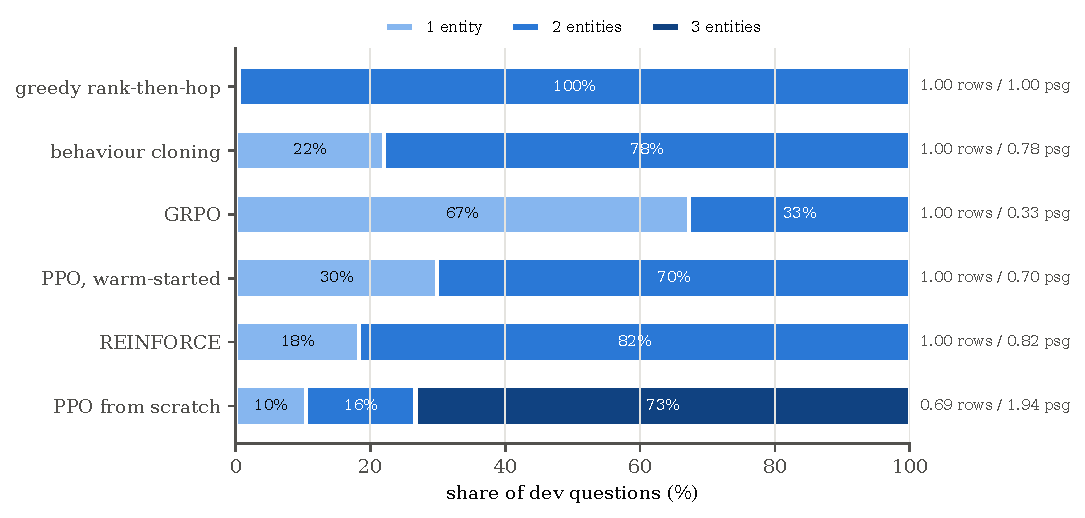
\includegraphics[width=0.92\textwidth]{figures/sizes.pdf}
\caption{Number of entities each selector passes to the reader on the dev set (learned selectors pooled over seeds), with the average numbers of rows and passages on the right.}
\label{fig:sizes}
\end{figure}

Selecting more entities is not, by itself, what makes the difference. Figure~\ref{fig:tradeoff} places every selector by the amount of text it passes to the reader. PPO from scratch uses about as many words as BM25 top-3 (\wordsScratch{} against \wordsBmThree{}), but scores \dScratchBm{} F1 more; taking more entities from any heuristic ranking helps much less. Within the warm-started family the entity cost has little room to act: for $c$ between 0 and 0.1 the evidence length stays between 151 and 169 words, with no monotone trend beyond $c=0$, and F1 varies by less than one point.

\begin{figure}[t]
\centering
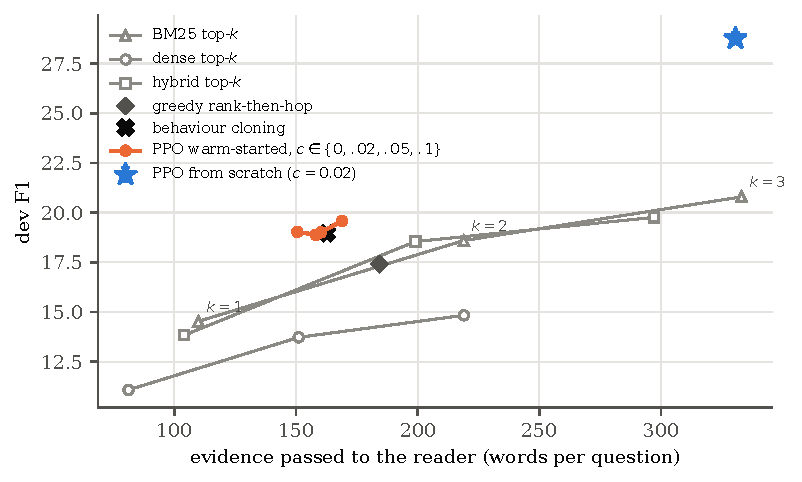
\includegraphics[width=0.85\textwidth]{figures/tradeoff.pdf}
\caption{Dev F1 against the evidence passed to the reader. Grey: top-$k$ heuristics for $k=1,2,3$. Orange: warm-started PPO with entity cost $c\in\{0,0.02,0.05,0.1\}$ (seeds 0--2). Blue star: PPO from scratch (three seeds; bar: standard deviation).}
\label{fig:tradeoff}
\end{figure}

\section{Learning dynamics}
\label{sec:dynamics}

Figure~\ref{fig:curves} shows validation F1 during training and Figure~\ref{fig:diagnostics} the training diagnostics; Table~\ref{tab:optim} summarises them.

\begin{figure}[t]
\centering
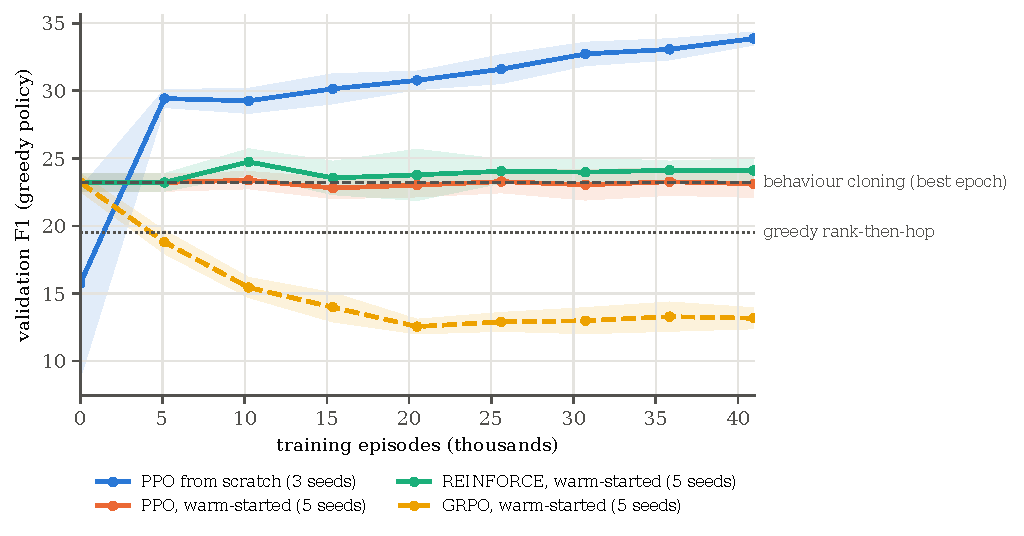
\includegraphics[width=0.9\textwidth]{figures/curves.pdf}
\caption{Validation F1 of the greedy policy during training (mean over seeds; band: $\pm$ one standard deviation). Every method sees 1{,}024 episodes per iteration. Episode~0 is the starting policy: the cloned policy for the warm-started methods, a random network for PPO from scratch.}
\label{fig:curves}
\end{figure}

\paragraph{PPO from scratch.} The randomly initialised policy starts at \initScratch{} validation F1, passes every other selector within the first five iterations, and is still improving when training stops (best validation F1 \valScratch{}, reached at the last iteration for all three seeds). Its sampled training F1 and its greedy validation F1 stay close (0.36 and 0.34 at the end), and its critic reaches an explained variance of about \evScratch{}. Over training the policy uses slightly fewer entities (from 2.86 to \itemsEndScratch{} per episode) and ends more episodes with an explicit \STOP{} (from 9\% to 22\%), which is the per-entity cost at work.

\paragraph{Warm-started PPO and REINFORCE.} Both start from the cloned policy at \initPpo{} validation F1. PPO's mean curve stays within one point of it, and REINFORCE gains one to two points. Their critics learn well (explained variance \evPpo{} and \evReinforce{}), and their sampled training F1 rises from 0.22 to 0.28--0.29, but the greedy validation score hardly follows. The policy updates are small: PPO's mean approximate KL per update is 0.003 and only 3\% of ratios are clipped, against 0.006 and 8\% for PPO from scratch, and the policy entropy falls from 0.80 to 0.40 nats. In words, the warm-started policies become more certain of the choices behaviour cloning taught them, and the improvement on training questions does not transfer. Behaviour cloning itself overfits: averaged over the five seeds, its training accuracy on oracle steps rises from 0.51 to 0.82 over eight epochs, while its validation loss is lowest after the third epoch and rises afterwards.

\paragraph{GRPO.} GRPO's validation F1 falls from \initGrpo{} to about 13 within twenty iterations, and the number of entities per episode collapses from 1.7 to \itemsEndGrpo. On average \degenGrpo\% of its groups receive identical returns and therefore no gradient. We think the collapse comes from the remaining groups. When the four answers of a group are equally wrong, the returns differ only through the per-entity cost, and dividing by the small within-group standard deviation turns differences of 0.02 into advantages of order one, which teaches the policy to stop as early as possible. We did not log per-group answer scores, so this explanation is an inference from the collapse in entity counts, not a measurement. It is the failure mode \citet{liu2025understanding} attribute to standard-deviation normalisation, and it matches the advantage collapse reported by \citet{wang2026igpo}.

\paragraph{Checkpoint selection.} The validation evaluation at iteration 5 happens before any actor update of the warm-started methods, because their critic-only warm-up lasts five iterations. For the iterate chosen at iteration 5, the reported model is therefore the cloned policy itself. This happened for PPO seed~0 among the main runs and for one or two seeds of several ablations (the ``Best it.'' column of Table~\ref{tab:ablation}); in all of these cases no later PPO iterate scored higher on validation, so the choice reflects the flat learning curves rather than changing the conclusions.

\begin{figure}[t]
\centering
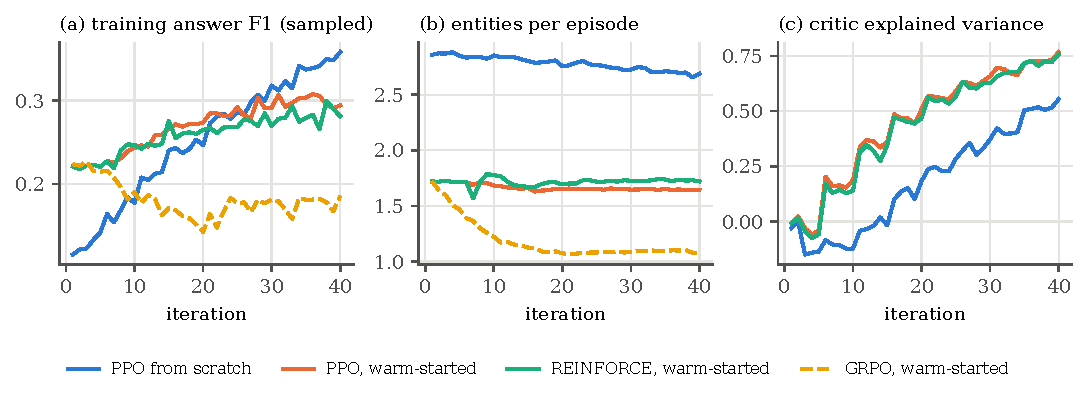
\includegraphics[width=\textwidth]{figures/diagnostics.pdf}
\caption{Training diagnostics per iteration, averaged over seeds: (a) F1 of the sampled episodes on training questions, (b) entities selected per episode, (c) explained variance of the critic (PPO and REINFORCE).}
\label{fig:diagnostics}
\end{figure}

\begin{table}[t]
\centering
\footnotesize
\caption{Training behaviour of the optimisers (same data, reward, evaluation and per-iteration episode budget). Init: initial validation F1 of the starting policy. Best val: validation F1 of the selected iterate (iteration in brackets, mean over seeds). EV: explained variance of the critic on the last batch. Items: entities per training episode at the last iteration. Time: minutes of training iterations per run (periodic validation excluded) on one T4 GPU.}
\label{tab:optim}
\setlength{\tabcolsep}{4pt}
\begin{tabular}{@{}lcccccc@{}}
\toprule
Method & Init & Best val (iter.) & Dev F1 & EV (end) & Items (end) & Time \\
\midrule
PPO + GAE from scratch & 15.8 & 33.9 (40) & 28.8\,{\scriptsize$\pm$0.3} & 0.55 & 2.69 & 2.2 \\
PPO + GAE, warm-started from BC & 23.2 & 23.7 (17) & 18.9\,{\scriptsize$\pm$0.4} & 0.77 & 1.64 & 1.7 \\
REINFORCE + baseline, warm-started & 23.2 & 25.1 (21) & 20.0\,{\scriptsize$\pm$0.5} & 0.76 & 1.72 & 1.2 \\
GRPO, warm-started & 23.2 & 18.8 (5) & 16.1\,{\scriptsize$\pm$0.5} & n/a & 1.08 & 0.9 \\
\bottomrule
\end{tabular}
\end{table}


\section{Reward and advantage ablations}
\label{sec:ablations}

Table~\ref{tab:ablation} varies the evidence term, the answer metric, the GAE parameter and the entity cost of the warm-started PPO configuration. All rows lie within 0.8 F1 of each other, which is about twice the seed standard deviation, and no setting moves the policy far from the cloned one. The largest values come from the settings that give the policy the most freedom or the noisiest signal, $c=0$ (19.6 F1) and $\lambda=1$ (19.5), but these differences are not significant at three seeds. The comparison between potential-based shaping and a terminal evidence bonus (G4) is therefore inconclusive in the warm-started regime: neither form changed what PPO learned, which is what the theory predicts for shaping but not necessarily for the bonus. The informative version of this experiment is to repeat it from scratch, where the policy does move (Chapter~\ref{ch:conclusion}).

\begin{table}[t]
\centering
\footnotesize
\caption{Ablations of the warm-started PPO configuration on the dev set (seeds 0--2 for every row, including the main configuration). Best it.: validation-selected iteration per seed. Path: a traced gold path is covered. R/L: exact match although no traced answer location is selected.}
\label{tab:ablation}
\setlength{\tabcolsep}{4pt}
\begin{tabular}{@{}llcccccc@{}}
\toprule
Factor & Setting & EM & F1 & Path & R/L & Items & Best it. \\
\midrule
Reward form & no evidence term & 14.1\,{\scriptsize$\pm$0.2} & 19.2\,{\scriptsize$\pm$0.1} & 36.7 & 0.1 & 1.73 & 5, 15, 25 \\
 & shaping, $\kappa=0.5$ (main) & 14.1\,{\scriptsize$\pm$0.4} & 19.0\,{\scriptsize$\pm$0.4} & 36.8 & 0.1 & 1.75 & 5, 10, 30 \\
 & terminal bonus, $\lambda_{\mathrm{ev}}=0.3$ & 14.2\,{\scriptsize$\pm$0.0} & 19.2\,{\scriptsize$\pm$0.1} & 37.4 & 0.1 & 1.75 & 15, 40, 20 \\
 & shaping, EM instead of F1 & 14.0\,{\scriptsize$\pm$0.3} & 19.0\,{\scriptsize$\pm$0.4} & 37.2 & 0.1 & 1.77 & 5, 20, 10 \\
\midrule
GAE $\lambda$ & $\lambda=0$ & 13.8\,{\scriptsize$\pm$0.4} & 18.8\,{\scriptsize$\pm$0.5} & 36.1 & 0.1 & 1.71 & 5, 35, 15 \\
 & $\lambda=0.95$ (main) & 14.1\,{\scriptsize$\pm$0.4} & 19.0\,{\scriptsize$\pm$0.4} & 36.8 & 0.1 & 1.75 & 5, 10, 30 \\
 & $\lambda=1$ & 14.5\,{\scriptsize$\pm$0.1} & 19.5\,{\scriptsize$\pm$0.2} & 37.9 & 0.1 & 1.77 & 10, 20, 20 \\
\midrule
Entity cost $c$ & $c=0$ & 14.5\,{\scriptsize$\pm$0.3} & 19.6\,{\scriptsize$\pm$0.4} & 38.3 & 0.1 & 1.81 & 10, 20, 25 \\
 & $c=0.02$ (main) & 14.1\,{\scriptsize$\pm$0.4} & 19.0\,{\scriptsize$\pm$0.4} & 36.8 & 0.1 & 1.75 & 5, 10, 30 \\
 & $c=0.05$ & 14.1\,{\scriptsize$\pm$0.3} & 19.0\,{\scriptsize$\pm$0.4} & 36.5 & 0.1 & 1.69 & 15, 10, 20 \\
 & $c=0.1$ & 14.0\,{\scriptsize$\pm$0.5} & 18.9\,{\scriptsize$\pm$0.6} & 36.4 & 0.1 & 1.74 & 5, 10, 5 \\
\bottomrule
\end{tabular}
\end{table}


\section{Generalisation checks}
\label{sec:unseen}

\paragraph{Unseen tables.} Because HybridQA's splits share tables, \testQuestionsWithTrainTable{} dev questions use a table that also occurs in our training subset. Table~\ref{tab:unseen} splits the dev set accordingly. On the questions whose table is unseen, PPO from scratch reaches \fScratchUnseen{} F1, against \fBcUnseen{} for behaviour cloning and \fBmThreeUnseen{} for BM25 top-3, so the gain does not depend on having seen the table.

\begin{table}[t]
\centering
\footnotesize
\caption{Dev results split by whether the question's table occurs in the training subset.}
\label{tab:unseen}
\begin{tabular}{@{}lcccc@{}}
\toprule
 & \multicolumn{2}{c}{Unseen tables (3,163 questions)} & \multicolumn{2}{c}{Seen tables (303 questions)} \\
\cmidrule(lr){2-3}\cmidrule(l){4-5}
Selector & EM & F1 & EM & F1 \\
\midrule
BM25 top-3 & 15.9 & 20.6 & 16.5 & 22.3 \\
Hybrid top-3 & 14.7 & 19.4 & 16.8 & 23.3 \\
Greedy rank-then-hop (HYBRIDER-style) & 12.8 & 17.4 & 13.9 & 17.7 \\
Behaviour cloning (BC) & 14.0\,{\scriptsize$\pm$0.3} & 18.8\,{\scriptsize$\pm$0.3} & 15.4\,{\scriptsize$\pm$0.5} & 20.7\,{\scriptsize$\pm$0.2} \\
GRPO, warm-started & 11.5\,{\scriptsize$\pm$0.3} & 15.9\,{\scriptsize$\pm$0.4} & 12.4\,{\scriptsize$\pm$0.8} & 17.5\,{\scriptsize$\pm$0.8} \\
PPO + GAE, warm-started from BC & 14.0\,{\scriptsize$\pm$0.4} & 18.8\,{\scriptsize$\pm$0.5} & 15.0\,{\scriptsize$\pm$0.8} & 20.4\,{\scriptsize$\pm$0.9} \\
REINFORCE + baseline, warm-started & 14.9\,{\scriptsize$\pm$0.5} & 19.9\,{\scriptsize$\pm$0.5} & 15.8\,{\scriptsize$\pm$1.0} & 21.3\,{\scriptsize$\pm$0.8} \\
PPO + GAE from scratch & 23.3\,{\scriptsize$\pm$0.2} & 28.6\,{\scriptsize$\pm$0.2} & 23.3\,{\scriptsize$\pm$1.0} & 30.7\,{\scriptsize$\pm$1.4} \\
Oracle gold path & 48.6 & 55.8 & 46.2 & 54.0 \\
\bottomrule
\end{tabular}
\end{table}


\paragraph{A second reader.} Table~\ref{tab:reader} keeps every selector's evidence fixed and replaces the reader by RoBERTa-base, which was never used in training, on the first 1{,}000 dev questions. The ranking of the selectors does not change. PPO from scratch reaches \robScratch{} F1 with the new reader, against \robBmThree{} for BM25 top-3, \robReinforce{} for REINFORCE and \robBc{} for behaviour cloning, while the oracle reaches \robOracle{}; most selectors gain a little from the stronger reader, and PPO from scratch gains slightly more than the others (from \miniScratch{} to \robScratch{} on these questions). The learned selection is therefore not tied to the quirks of the reader it was trained with. So that the table is internally consistent, all of its second-reader entries were computed in one environment (the laptop CPU) from the stored selections; as a check, re-reading behaviour cloning's seed-0 selections there gave 16.0 EM / 20.4 F1, against 15.8 / 20.2 in the GPU environment.

\begin{table}[t]
\centering
\footnotesize
\caption{Transfer to a second frozen reader (RoBERTa-base SQuAD~2.0) that was never used during training, on the first 1{,}000 dev questions (the dev file is ordered by a hashed question id). Each selector's evidence is exactly what it selected in the main evaluation; only the reader changes. The oracle is recomputed under the new reader. Left: the training reader's scores on the same questions.}
\label{tab:reader}
\begin{tabular}{@{}lcccc@{}}
\toprule
 & \multicolumn{2}{c}{Training reader (MiniLM)} & \multicolumn{2}{c}{Unseen reader (RoBERTa)} \\
\cmidrule(lr){2-3}\cmidrule(l){4-5}
Selector & EM & F1 & EM & F1 \\
\midrule
Dense top-2 (TableRAG-style) & 10.4 & 14.1 & 11.1 & 14.3 \\
Hybrid top-2 & 14.9 & 19.5 & 16.1 & 20.2 \\
Hybrid top-3 & 14.9 & 19.8 & 16.0 & 20.8 \\
BM25 top-3 & 15.9 & 20.5 & 16.5 & 21.1 \\
Greedy rank-then-hop (HYBRIDER-style) & 13.6 & 18.4 & 14.0 & 18.0 \\
Behaviour cloning (BC) & 13.8\,{\scriptsize$\pm$0.6} & 19.1\,{\scriptsize$\pm$0.5} & 16.0\,{\scriptsize$\pm$0.5} & 20.5\,{\scriptsize$\pm$0.3} \\
GRPO, warm-started & 10.9\,{\scriptsize$\pm$0.8} & 15.7\,{\scriptsize$\pm$0.9} & 12.0\,{\scriptsize$\pm$0.8} & 16.2\,{\scriptsize$\pm$1.0} \\
PPO + GAE, warm-started from BC & 13.5\,{\scriptsize$\pm$0.6} & 18.9\,{\scriptsize$\pm$0.7} & 15.3\,{\scriptsize$\pm$0.8} & 20.0\,{\scriptsize$\pm$0.8} \\
REINFORCE + baseline, warm-started & 15.0\,{\scriptsize$\pm$0.7} & 20.5\,{\scriptsize$\pm$0.7} & 16.3\,{\scriptsize$\pm$0.8} & 21.1\,{\scriptsize$\pm$0.8} \\
PPO + GAE from scratch & 23.7\,{\scriptsize$\pm$0.1} & 28.7\,{\scriptsize$\pm$0.0} & 25.5\,{\scriptsize$\pm$0.3} & 30.8\,{\scriptsize$\pm$0.5} \\
Oracle gold path & 49.0 & 56.7 & 54.2 & 61.4 \\
\bottomrule
\end{tabular}
\end{table}



\section{Compute}
\label{sec:compute}

Preparing the data (graph construction and embedding of 230{,}512 entity texts) took 5.2 hours on the laptop CPU, most of it under battery throttling. On the laptop, one reader call costs about 120~ms, so a single PPO run with the reader in the loop would take several hours. All reported training and evaluation therefore ran on one NVIDIA T4 GPU, where the complete suite (baselines, 5 behaviour-cloning runs, 42 reinforcement-learning runs, all dev evaluations and the second-reader experiment) took 1.17 hours. A PPO run of 40 iterations takes 1--3 minutes there (Table~\ref{tab:optim}), most of it Python-side environment stepping; the policy itself is too small to matter. The decomposable reader and its cache are what make this possible: every (question, entity) pair is read once and reused by all methods, seeds and iterations.

\chapter{PLACEHOLDER discussion}
\label{ch:discussion}
PLACEHOLDER

\chapter{PLACEHOLDER conclusion}
\label{ch:conclusion}
PLACEHOLDER


\bibliographystyle{plainnat}
\bibliography{references}

\appendix
\chapter{Reproducing the Experiments}
\label{app:repro}

All commands are run from the repository root with Python~3.12; the package versions are pinned in \texttt{requirements.txt}. Every step writes its outputs under \texttt{data/} or \texttt{results/}, and the last two steps regenerate every table and figure of Chapter~\ref{ch:results} directly into the \LaTeX{} sources.

\begin{small}
\begin{verbatim}
# 1. data (HybridQA questions + WikiTables-WithLinks tables and passages)
git clone --depth 1 https://github.com/wenhuchen/HybridQA data/raw/HybridQA
git clone --depth 1 --no-checkout https://github.com/wenhuchen/WikiTables-WithLinks \
          data/raw/WikiTables-WithLinks
python scripts/extract_wikitables.py          # reads blobs from the git object store
python scripts/build_instances.py --n_train 10000 --n_val 1000
python scripts/data_stats.py
python tests/test_core.py                      # unit tests

# 2. baselines with the frozen reader
python scripts/run_baselines.py --split val
python scripts/run_baselines.py --split test

# 3. learned selectors (one command per seed)
python scripts/train.py --method bc --seed 0
python scripts/train.py --config configs/ppo_main.yaml --seed 0
python scripts/train.py --config configs/grpo.yaml --seed 0
python scripts/train.py --config configs/reinforce.yaml --seed 0
#    ablations: configs/ppo_{noshape,evbonus,em,lam0,lam1,nocost,cost05,cost10,scratch}.yaml

# 4. evaluation, second reader, tables and figures
python scripts/evaluate.py --runs results/runs/* --split test
python scripts/run_baselines.py --split test --reader deepset/roberta-base-squad2 --limit 1000
python scripts/evaluate.py --runs results/runs/* --split test \
                           --reader deepset/roberta-base-squad2 --limit 1000
python scripts/make_assets.py
\end{verbatim}
\end{small}

\chapter{Repository Layout}
\label{app:layout}

\begin{small}
\begin{verbatim}
configs/            one YAML file per experiment (reward, environment, optimiser)
data/               raw clones, processed graphs and embeddings, reader cache (not versioned)
docs/               earlier planning documents of the project
papers/             PDFs of the papers collected in the first phase
report/             this report (main.tex, chapters/, generated/, figures/, references.bib)
reports/            literature synthesis that the review chapters are based on
research_notes/     per-topic notes of the literature search, with verified BibTeX
results/            baselines/, runs/<name>_s<seed>/, logs/, summary files
scripts/            command-line entry points listed in Appendix A
src/mhtrl/          data, environment, policy, reader, rollout, rl/ (PPO, GRPO, REINFORCE, BC)
tests/              unit tests
\end{verbatim}
\end{small}


\end{document}
